\documentclass[landscape,fleqno]{foils}

\usepackage{ae}
%\usepackage{hyperref}
%\usepackage{thumbpdf}
\usepackage{graphicx}
\usepackage{color}
\usepackage[left=1cm,right=1cm,top=2cm,bottom=2cm]{geometry}
% \usepackage[display]{texpower}
%\usepackage{psfrag}
\usepackage{ragged2e}
\usepackage{amstext}
\usepackage{xspace}
\usepackage{fancyvrb}
\usepackage{amsmath}
\usepackage{url}
\usepackage{pause}
\usepackage{tabularx}

\newcommand{\figfigure}[2]{%
  \begin{psfrags}%
  \input #2.eps_t%
  \includegraphics[width=#1]{#2.eps}%
  \end{psfrags}%
}

\newcommand{\stitle}[1]{{\color{blue}\Large #1\par\vspace*{10pt}\hrule}}
\newcommand{\cstitle}[1]{{\centering\color{blue}\Large #1\par\vspace*{10pt}\hrule}}

\setlength{\columnsep}{0.5cm}
\setlength{\columnseprule}{0.4pt}

\renewcommand{\emph}[1]{\textcolor{red}{\bf #1}}

\newcommand{\igraph}{\texttt{{igraph}}\xspace}

\DefineVerbatimEnvironment{Myverb}{Verbatim}
{gobble=2,numbers=left,numbersep=5mm,frame=lines,fontsize=\small}

\newenvironment{narrow}[2]{%
  \begin{list}{}{%
      \setlength{\topsep}{0pt}%
      \setlength{\leftmargin}{#1}%
      \setlength{\rightmargin}{#2}%
      \setlength{\listparindent}{\parindent}%
      \setlength{\itemindent}{\parindent}%
      \setlength{\parsep}{\parskip}}%
    \item[]}{\end{list}}

\newcommand{\bull}{$\bullet$\xspace}

\begin{document}

\RaggedRight
% \color{white}
% \pagecolor{black}
\fvset{fontsize=\small}
\fvset{commandchars=\\\{\}}
\definecolor{grey}{gray}{0.75}
\fvset{frame=single, numbers=left, rulecolor=\color{grey}}

\MyLogo{\color{black}\texttt{http://cneurocvs.rmki.kfki.hu/igraph/NIPS2008.html}}

\thispagestyle{empty}
\vspace*{1cm}
{\centering
\hrule
\Large
\vspace*{1cm}
{\bf Large-scale network analysis}
\vspace*{1cm}
\par
\hrule
\par
\vspace*{2cm}
\normalsize G\'abor Cs\'ardi\\
\small \verb+csardi@rmki.kfki.hu+
\par
\vspace*{1.5cm}
Department of Biophysics, 
KFKI Research Institute for Nuclear and Particle Physics of the\\
Hungarian Academy of Sciences, Budapest, Hungary\\[15pt]
Currently at \\Department of Medical Genetics, \\
University of Lausanne, Lausanne, Switzerland\\
}

\newpage
\stitle{Outline}

\begin{enumerate}
{\centering
\item The igraph R package\par
\item What can you do with large graphs?\par
\item Some unique igraph features\par
\item Rapid prototyping\par
}
\end{enumerate}

\newpage
\stitle{The \emph{igraph} software package}

\begin{itemize}
\item R package, Python extension and C library. \pause
\item Under active development. \pause
\item Free for academic and commercial use (GPL). ``Standing on the
  shoulder of giants.'' \pause
\item State of the art data structures and algorithms, works well with
  large graphs.
\end{itemize}

\newpage
\stitle{How \emph{LARGE}?}

\begin{itemize}
\item Well, it depends what you want to calculate. \pause
\item Just to create and manipulate it, it is enough
  if it fits into the memory. \pause
\item How do I know that it fits into the memory? \pause
\item igraph (typically) needs 32 bytes per edge and 16 bytes per
  vertex. \pause
\item A graph with one million vertices and ten million edges needs 
  about 320 Mbytes.
\end{itemize}

\newpage
\stitle{Installation}

\begin{Myverb}
  install.packages("igraph")
\end{Myverb}

It is really that simple. Isn't it? \pause
\vspace*{2cm}

You might also need\vspace*{-1cm}
\begin{Myverb}
  install.packages("digest")
  install.packages("rgl")
\end{Myverb}

\newpage
\stitle{How to follow this ``lecture''?}
\begin{enumerate}
%\item Type 
%\begin{Myverb}
%  source("http://cneurocvs.rmki.kfki.hu/igraph/NIPS2008.R")
%\end{Myverb}
%and everything is run for you. You will see the commands on the screen
%before R actually runs them, and you'll need to press \verb+ENTER+ to
%proceed.\pause
\item Go to \textcolor{red}{\url{http://cneurocvs.rmki.kfki.hu/igraph/NIPS2008.html}} and 
  copy \& paste everything into your R session. You can skip any
  example if you wish to.
  \pause
\item You type in everything I type in. \pause
\item Sit back and watch. You can download the slides/code anyway.
\end{enumerate}

\newpage
\stitle{The igraph data model}
\begin{itemize}
\item Binary relation (=\emph{edges}) between elements of a set
  (=\emph{vertices}). \pause\\[-15pt]
\item If the pairs are unordered, then the graph is undirected:\\[-20pt]

  \begin{minipage}{0.7\textwidth}
    \begin{align} 
      \text{vertices} & =\{A,B,C,D,E\} \nonumber\\
      \text{edges}    & =( \{A,B\},\{A,C\},\{B,C\},\{C,E\} ). \nonumber
    \end{align}
  \end{minipage}\begin{minipage}{0.3\textwidth}
    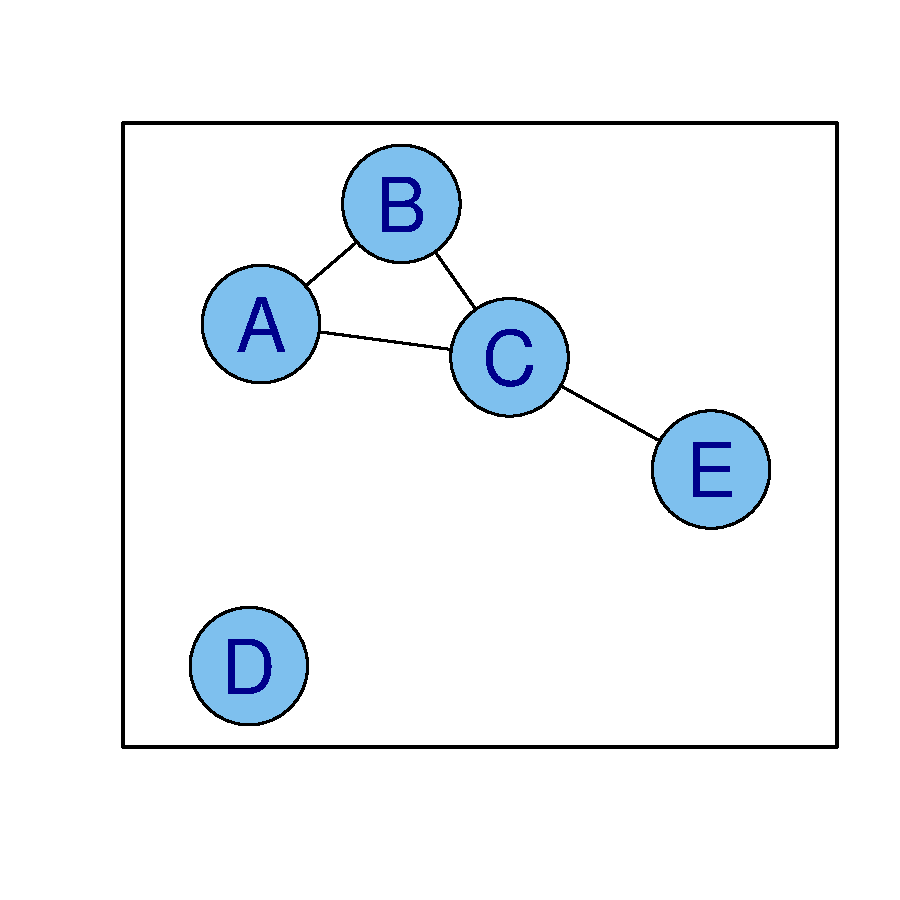
\includegraphics[width=0.8\textwidth]{../images/small3}
  \end{minipage}\pause
\item Otherwise it is directed:\\[-20pt]

  \begin{minipage}{0.7\textwidth}
    \begin{align} 
      \text{vertices} & =\{A,B,C,D,E\} \nonumber\\
      \text{edges}    & =( (A,B),(A,C),(B,C),(C,E) ). \nonumber
    \end{align}
  \end{minipage}\begin{minipage}{0.3\textwidth}
    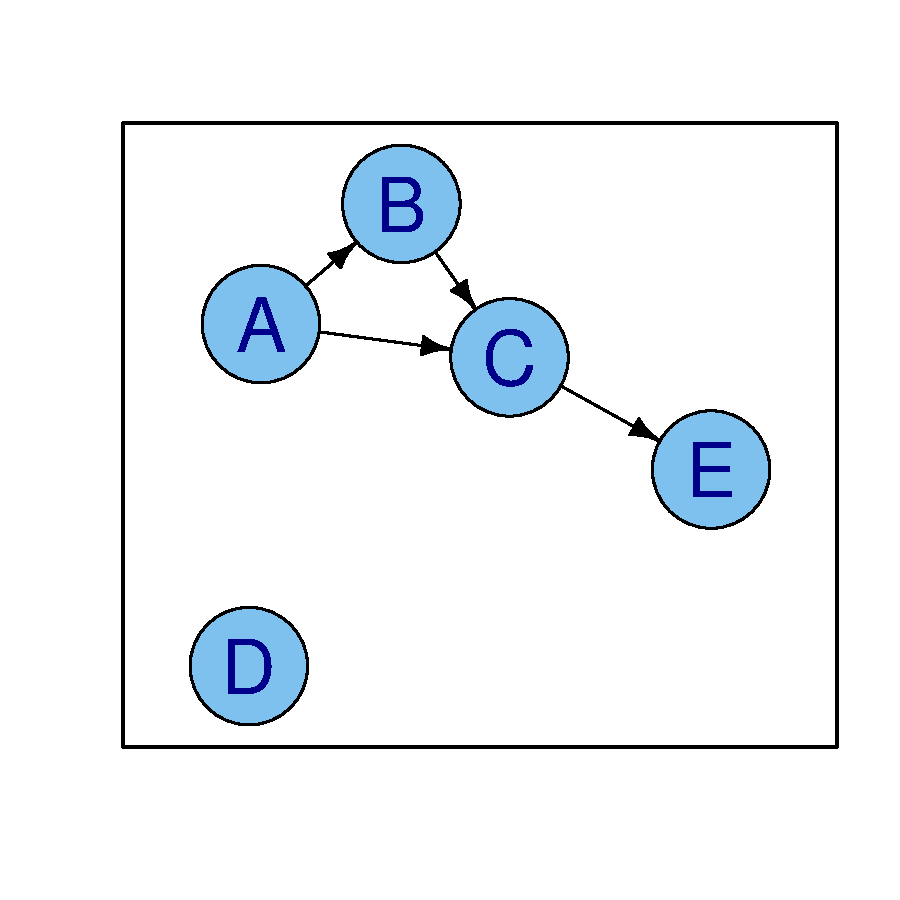
\includegraphics[width=0.8\textwidth]{../images/small4}
  \end{minipage}
\end{itemize}

\newpage
\stitle{Vertex and edge ids}
\begin{narrow}{0cm}{13.5cm}
\begin{itemize}
\item Vertices are always numbered from 0.
\item Numbering is continual, form 0 to $n-1$. \pause
\item We have to translate vertex names to ids: 
\begin{align} 
  V & =\{A,B,C,D,E\} \nonumber\\
  E & =( (A,B),(A,C),(B,C),(C,E) ). \nonumber\\
  A & =0, B=1, C=2, D=3, E=4. \nonumber
\end{align}\vspace*{-2cm}\pause
\begin{Myverb}
  library(igraph)
  g <- graph( c(0,1, 0,2, 1,2, 2,4), n=5 )
  g
  g2 <- graph( c(0,1, 0,2, 1,2, 2,4), 
               n=5, dir=FALSE )
  g2
\end{Myverb}
\end{itemize}
\end{narrow}

\newpage
\stitle{Working with igraph graphs}
\begin{Myverb}
  ## How to decide what kind of object a variable refers to
  class(g2)
  class(1)
  class("foobar")

  ## Is this object an igraph graph?
  is.igraph(g)
  is.igraph(1:10)

  ## Summary, number of vertices, edges
  summary(g)
  vcount(g)
  ecount(g)

  ## Is the graph directed?
  is.directed(g)
  is.directed(g2)
  is.directed(1:10)
\end{Myverb}

\newpage
\stitle{Working with igraph graphs}
\begin{Myverb}
  ## Convert from directed to undirected
  as.undirected(g)

  ## And back
  as.directed(as.undirected(g))
\end{Myverb}

\newpage
\stitle{The igraph data model, multiple edges}
\begin{narrow}{0cm}{15cm}
\begin{itemize}
\item \igraph can handle multi-graphs:
  \begin{align} 
    V & =\{A,B,C,D,E\} \nonumber\\
    E & =( (AB),(AB),(AC),(BC),(CE) ). \nonumber
  \end{align}
  \begin{Myverb}
  g <- graph( c(0,1,0,1, 0,2, 1,2, 3,4), n=5 )
  g
  \end{Myverb}
\end{itemize}
\end{narrow}

\newpage
\stitle{The igraph data model, loop edges}
\begin{narrow}{0cm}{15cm}
\begin{itemize}
\item \igraph can handle loop-edges:
  \begin{align} 
    V & =\{A,B,C,D,E\} \nonumber\\
    E & =( (AA),(AB),(AC),(BC),(CE) ). \nonumber
  \end{align}
  \begin{Myverb}
  g <- graph( c(0,0,0,1, 0,2, 1,2, 3,4), n=5 )
  g
  \end{Myverb}
\end{itemize}
\end{narrow}

\newpage
\stitle{The igraph data model, what cannot be represented}
\begin{itemize}
\item ``Mixed'' graphs, with undirected and directed edges.
\item Hypergraphs.
\item No direct support for bipartite (two-mode) graphs.
\end{itemize}

% \newpage
% \stitle{Creating graphs, using vertex ids}
% \begin{narrow}{0cm}{15cm}
% \end{narrow}

\newpage
\stitle{Naming vertices}
\begin{narrow}{0cm}{15cm}
\begin{Myverb}
  g <- graph.ring(10)
  V(g)$name <- letters[1:10]
  V(g)$name
  g
  print(g, v=T)
\end{Myverb}
\end{narrow}

\newpage
\stitle{Creating graphs, the formula interface}
\begin{narrow}{0cm}{15cm}
\begin{Myverb}
  # A simple undirected graph
  g <- graph.formula( Alice-Bob-Cecil-Alice, 
       Daniel-Cecil-Eugene, Cecil-Gordon )
\end{Myverb}
\vspace*{-2cm} \pause
\begin{Myverb}
  # Another undirected graph, ":" notation
  g2 <- graph.formula( Alice-Bob:Cecil:Daniel, 
       Cecil:Daniel-Eugene:Gordon )
\end{Myverb}
\vspace*{-2cm} \pause
\begin{Myverb}
  # A directed graph
  g3 <- graph.formula( Alice +-+ Bob --+ Cecil 
      +-- Daniel, Eugene --+ Gordon:Helen )
\end{Myverb}
\vspace*{-2cm} \pause
\begin{Myverb}
  # A graph with isolate vertices
  g4 <- graph.formula( Alice -- Bob -- Daniel, 
      Cecil:Gordon, Helen )
\end{Myverb}
\vspace*{-2cm} \pause
\begin{Myverb}
  # "Arrows" can be arbitrarily long
  g5 <- graph.formula( Alice +---------+ Bob )
\end{Myverb}
\end{narrow}

\newpage
\stitle{Creating graphs, from edge lists and adjacency matrices}
\begin{Myverb}
  ## From edge lists
  el <- cbind( c(0, 0, 1, 2),
               c(1, 2, 2, 4) )
  g <- graph.edgelist(el)
  g

  ## Symbolic edge lists
  el <- cbind( c("Alice", "Alice", "Bob",   "Cecil"),
               c("Bob",   "Cecil", "Cecil", "Ed") )
  g <- graph.edgelist(el)
  g
  summary(g)

  ## Adjacency matrices
  A <- matrix(sample(0:1, 100, rep=TRUE), 10, 10)
  g <- graph.adjacency(A)
\end{Myverb}

\newpage
\stitle{Creating graphs, from data frames}
%% Here we start the example from Fowler's paper
%% use the new version of graph.data.frame and read.csv

\begin{narrow}{0cm}{15cm}
\begin{Myverb}
  source("http://cneurocvs.rmki.kfki.hu/igraph/plus.R")
  vertices <- read.csv("judicial.csv")
  edges <- read.table("allcites.txt")
  jg <- graph.data.frame(edges, vertices=vertices, dir=TRUE)
\end{Myverb}
\end{narrow}

\newpage
\stitle{Visualizing graphs}
\begin{narrow}{0cm}{15cm}
\begin{itemize}
\item \verb+plot+ Uses traditional R graphics, non-interactive, 2d.
  Publication quality plots in all formats R supports. \pause
\begin{Myverb}
  g <- barabasi.game(100, m=1)
  g <- simplify(g)
  igraph.par("plot.layout", 
             layout.fruchterman.reingold)
  plot(g, vertex.size=3, vertex.label=NA, 
       edge.arrow.size=0.6)
\end{Myverb}
\end{itemize}
\end{narrow}

\newpage
\stitle{Visualizing graphs}
\begin{narrow}{0cm}{15cm}
\begin{itemize}
\item \verb+tkplot+ Uses Tcl/Tk via the \verb+tcltk+ package, 
  interactive, 2d. \pause
\begin{Myverb}
  id <- tkplot(g, vertex.size=3, vertex.label=NA, 
        edge.arrow.size=0.6)
  coords <- tkplot.getcoords(id)
\end{Myverb}
\pause
\item \verb+rglplot+ Needs the \verb+rgl+ package. \pause
\begin{Myverb}
  rglplot(g, vertex.size=3, vertex.label=NA)

  coords <- layout.kamada.kawai(g, dim=3)
  rglplot(g, vertex.size=3, vertex.label=NA, 
          layout=coords)
\end{Myverb}
\pause
\item (Almost) identical interfaces.
\end{itemize}
\end{narrow}

\newpage
\stitle{Graph/vertex/edge attributes}
\begin{narrow}{0cm}{15cm}
\begin{itemize}
\item Assigning/querying attributes:
  {\small
    \texttt{set.graph.attribute},~\texttt{get.graph.attribute},
    \texttt{set.vertex.attribute},~\texttt{get.vertex.attribute},  
    \texttt{set.edge.attribute},~\texttt{get.edge.attribute},
    \texttt{list.graph.attributes},
    \texttt{list.vertex.attributes},
    \texttt{list.edge.attributes}.
} \pause
\item \verb+V(g)+ and \verb+E(g)+. \pause
\end{itemize}
\end{narrow}

\newpage
\stitle{Graph/vertex/edge attributes}
\begin{Myverb}
  ## Load the jurisdiction network
  load("judicial.Rdata.gz")

  ## If we don't have it then create it again
  if (!exists("jg")) \{
    source("http://cneurocvs.rmki.kfki.hu/igraph/plus.R")
    vertices <- read.csv("http://cneurocvs.rmki.kfki.hu/igraph/judicial.csv")
    edges <- read.table("http://cneurocvs.rmki.kfki.hu/igraph/allcites.txt")
    jg <- graph.data.frame(edges, vertices=vertices, dir=TRUE)
  \}
\end{Myverb}

\newpage
\stitle{Graph/vertex/edge attributes}
\begin{Myverb}
  ## What do we have?
  summary(jg)
  V(jg)$year
  V(jg)$parties

  ## Select vertices based on attributes
  V(jg) [ year >= 1990 ]
  V(jg) [ overruled!=0 ]

  ## Group network measures based on attributes
  deg.per.year <- tapply(degree(jg, mode="out"), 
                  V(jg)$year, mean)

  ## Plot it
  plot( names(deg.per.year), deg.per.year )
\end{Myverb}

\newpage
\stitle{Smart indexing}
\begin{narrow}{0cm}{15cm}
\begin{itemize}
\item Easy access of attributes:
  \begin{Myverb}
  g <- erdos.renyi.game(100, 1/100)
  V(g)$color <- sample( c("red", "black"), 
                          vcount(g), rep=TRUE)
  E(g)$color <- "grey"
  red <- V(g)[ color == "red" ]
  bl <- V(g)[ color == "black" ]
  E(g)[ red %--% red ]$color <- "red"
  E(g)[ bl  %--% bl ]$color <- "black"
  plot(g, vertex.size=5, layout=
         layout.fruchterman.reingold)
\end{Myverb}
\end{itemize}
\end{narrow}

\newpage
\stitle{Centrality, the network}
\begin{Myverb}
  g <- graph.formula( Andre----Beverly:Diane:Fernando:Carol,
                      Beverly--Andre:Diane:Garth:Ed,
                      Carol----Andre:Diane:Fernando,
                      Diane----Andre:Carol:Fernando:Garth:Ed:Beverly,
                      Ed-------Beverly:Diane:Garth,
                      Fernando-Carol:Andre:Diane:Garth:Heather,
                      Garth----Ed:Beverly:Diane:Fernando:Heather,
                      Heather--Fernando:Garth:Ike,
                      Ike------Heather:Jane,
                      Jane-----Ike )
  g <- simplify(g)
  coords <- c(5,5,119,256,119,256,120,340,478,
      622,116,330,231,116,5,330,451,231,231,231)
  coords <- matrix(coords, nc=2)
  V(g)$label <- V(g)$name
  g$layout <- coords # $
  plot(g, asp=FALSE, vertex.label.color="blue", vertex.label.cex=1.5,
       vertex.label.font=2, vertex.size=20, vertex.color="white",
       vertex.frame.color="white", edge.color="black")  
\end{Myverb}

\newpage
\stitle{Centrality, the network}
\begin{center}
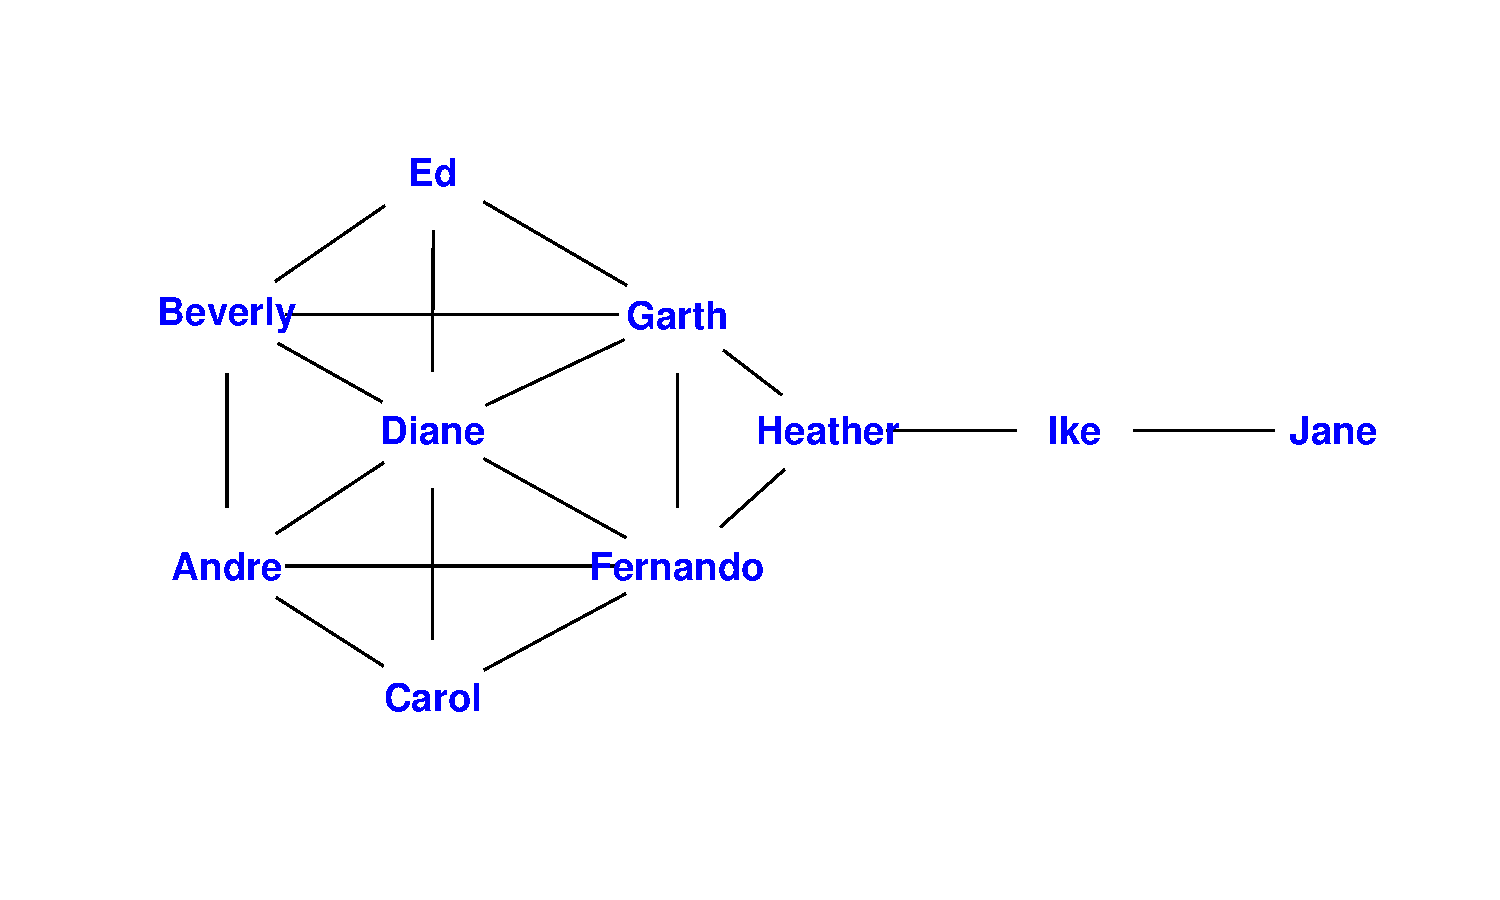
\includegraphics[width=0.8\textwidth]{centnet}
\end{center}    

\newpage
\stitle{Centrality, degree}
\begin{center}
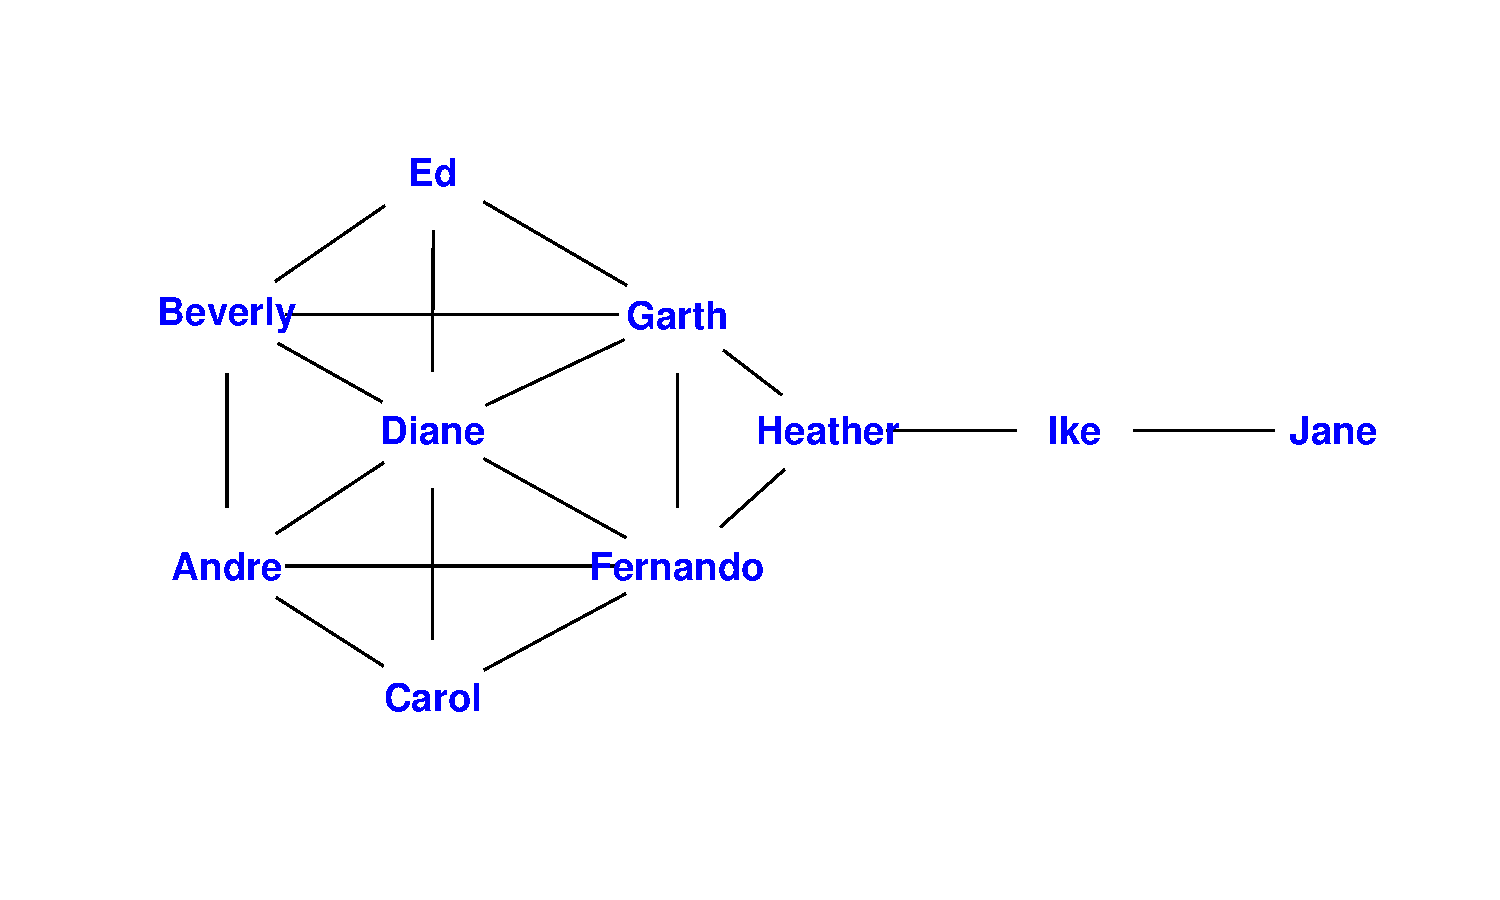
\includegraphics[width=0.8\textwidth]{centnet}
\par Number of adjacent edges.
\end{center}

\newpage
\stitle{Centrality, degree}
\begin{center}
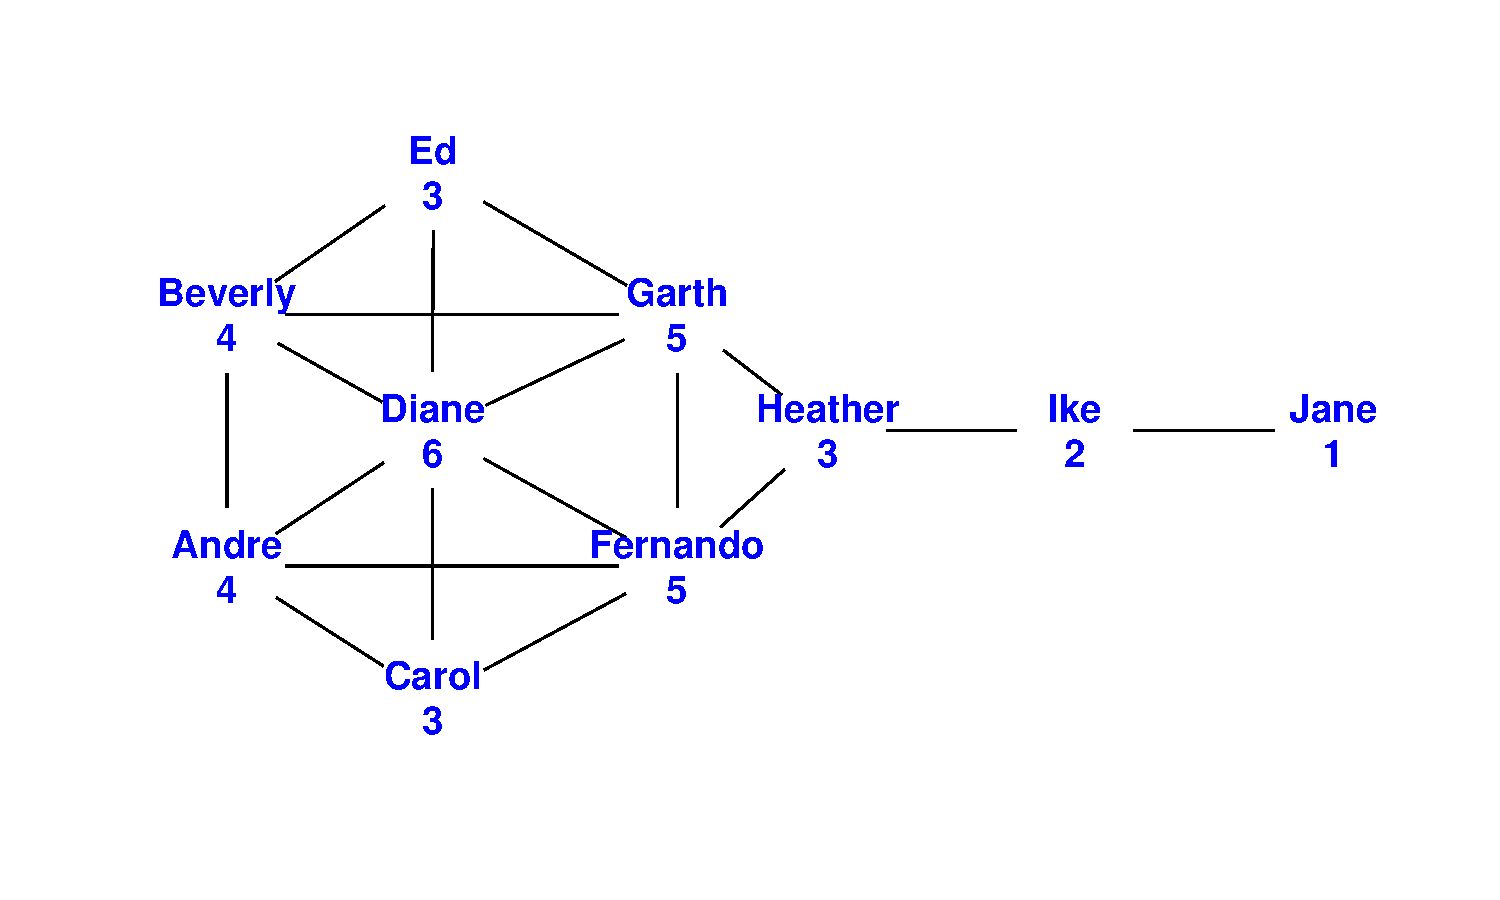
\includegraphics[width=0.8\textwidth]{centnet-degree}
\par Number of adjacent edges.
\end{center}

\newpage
\stitle{Centrality, closeness}
\begin{center}
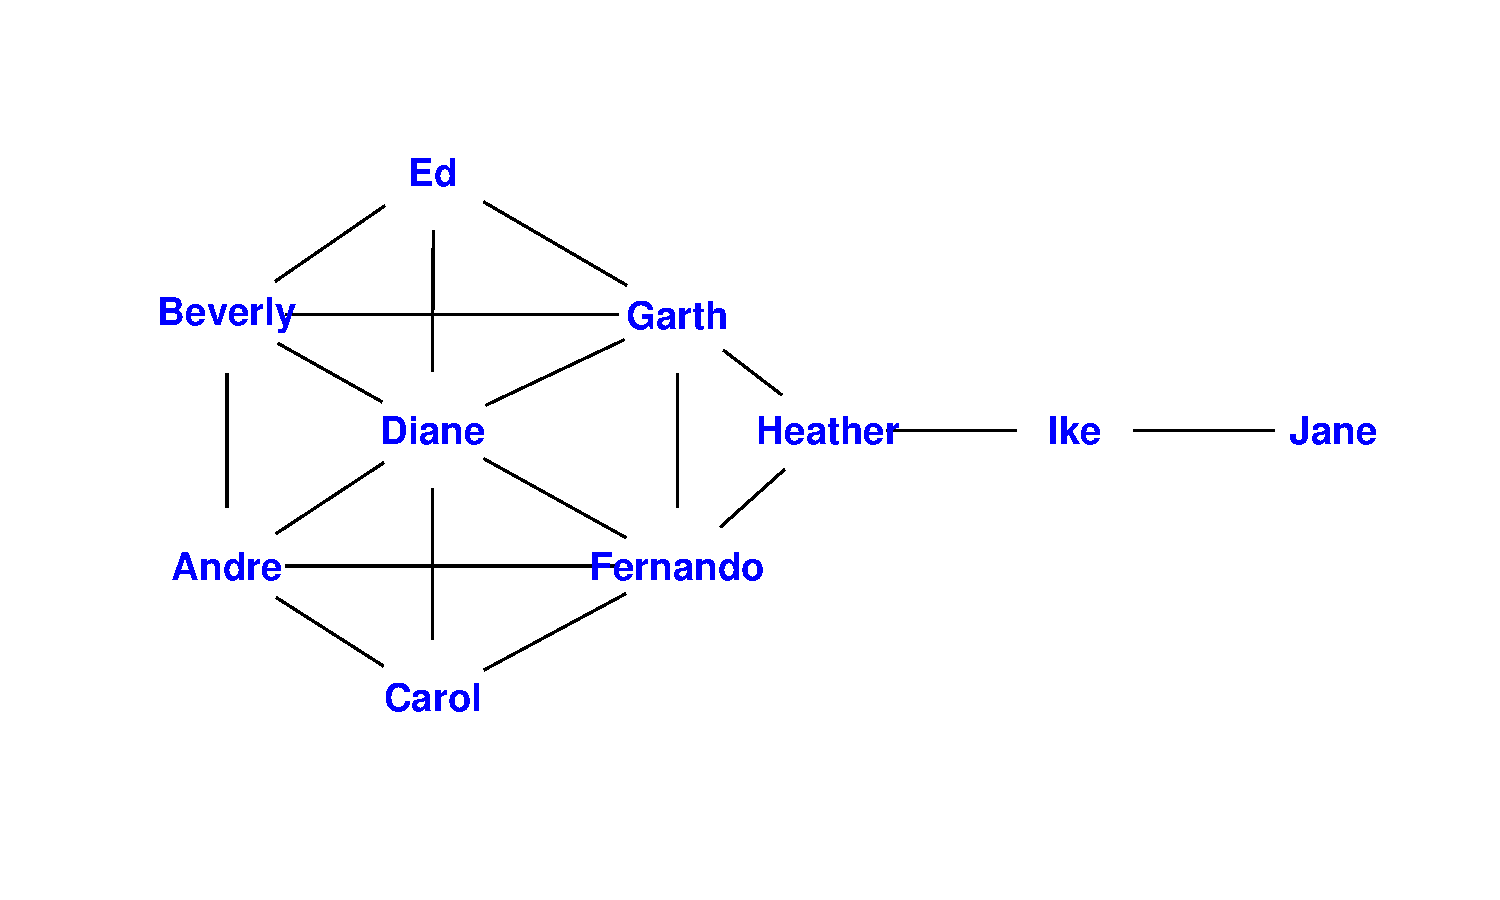
\includegraphics[width=0.8\textwidth]{centnet}
\par Reciproc of the average distance to other vertices.
\end{center}

\newpage
\stitle{Centrality, closeness}
\begin{center}
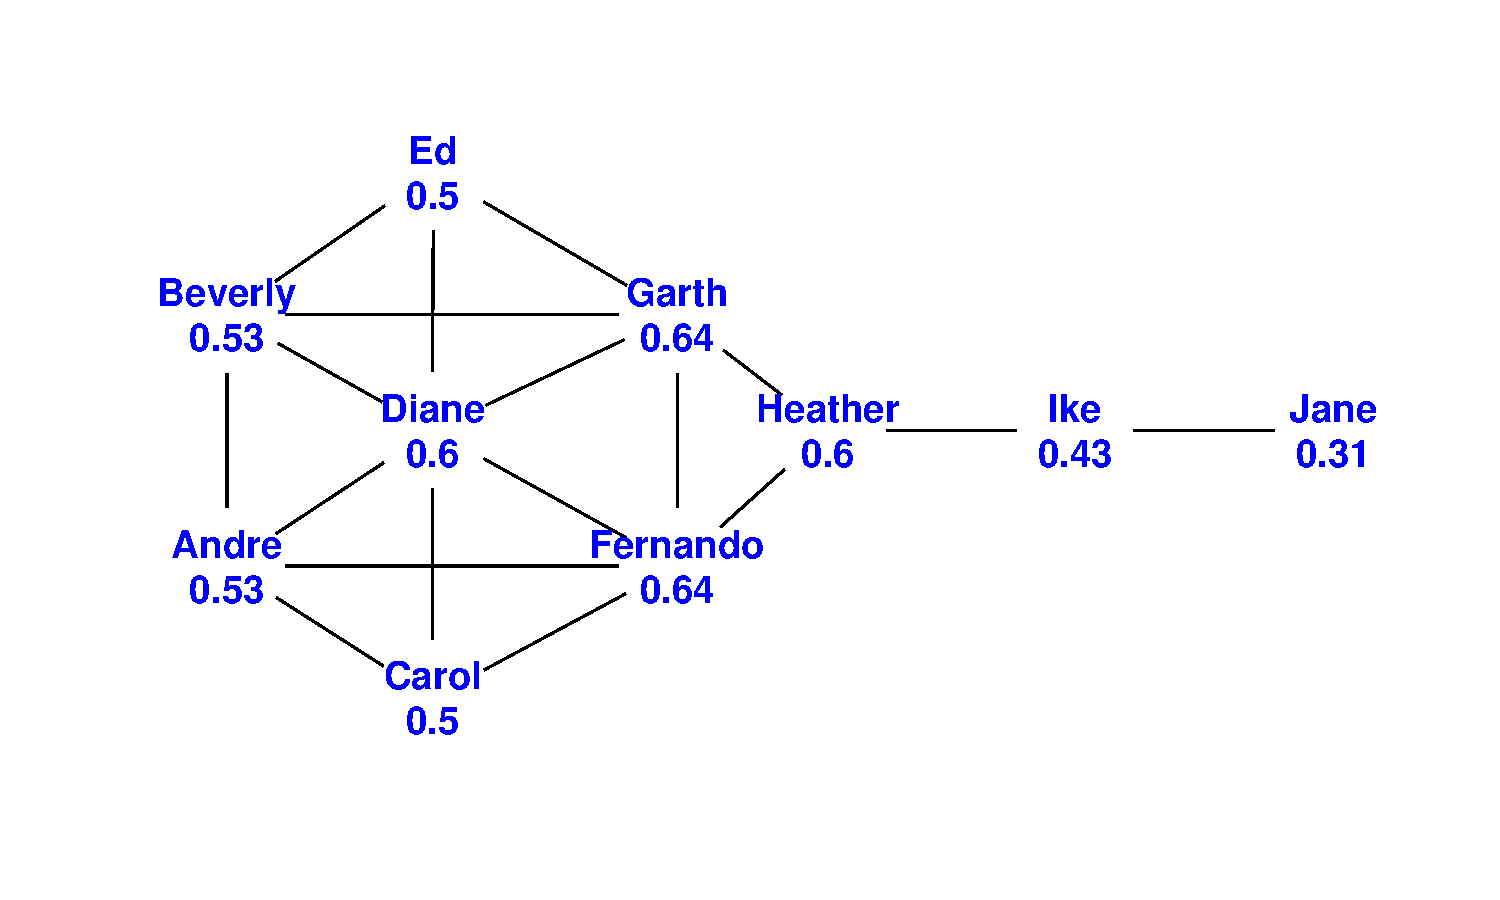
\includegraphics[width=0.8\textwidth]{centnet-closeness}
\par Reciproc of the average distance to other vertices.
\end{center}

\newpage
\stitle{Centrality, betweenness}
\begin{center}
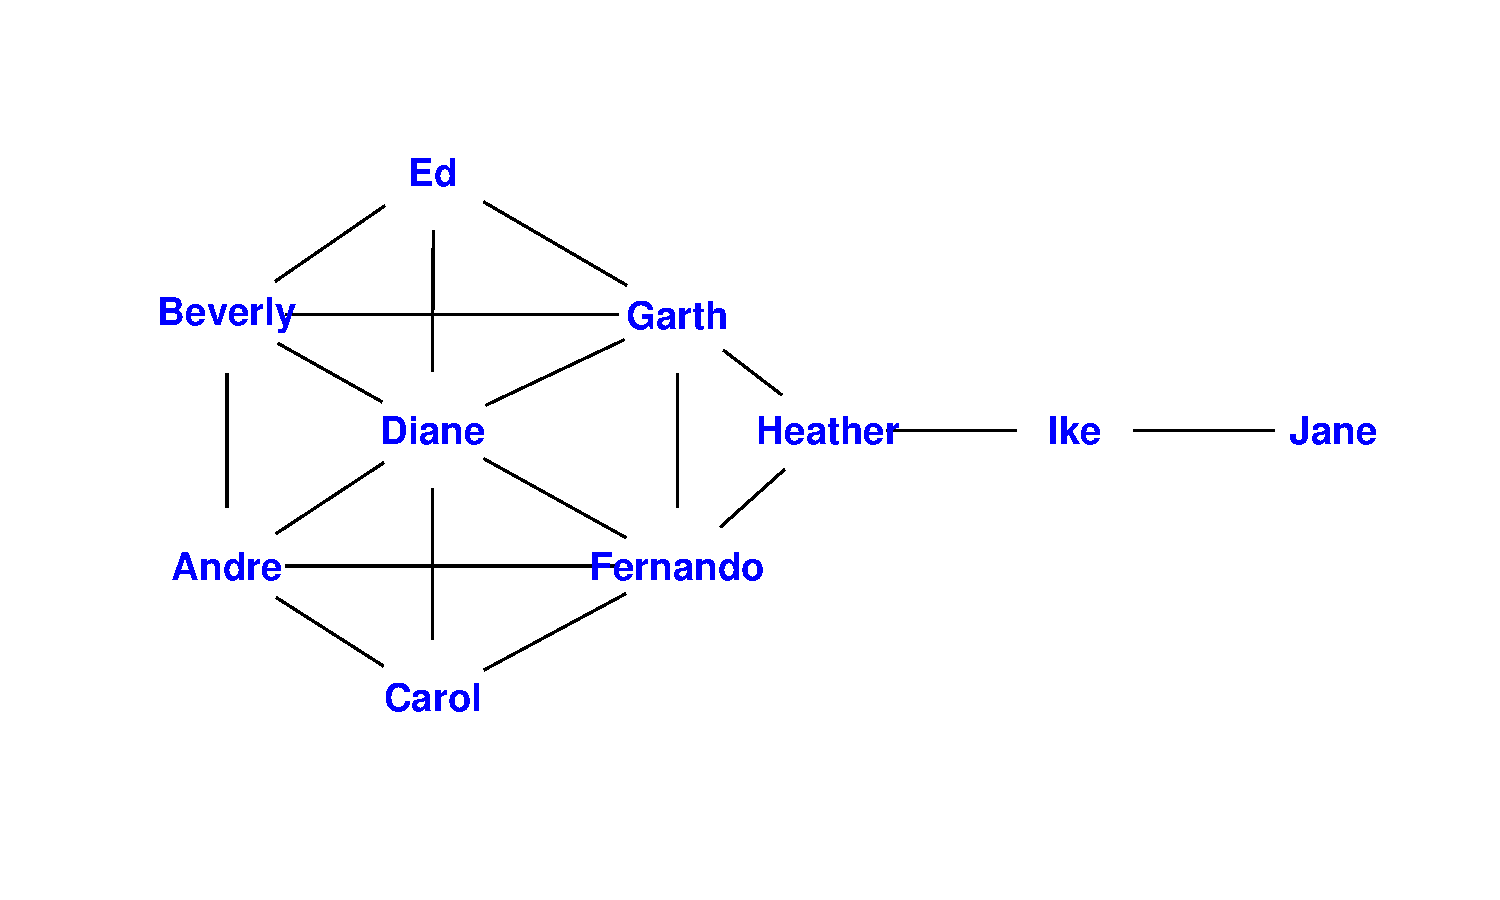
\includegraphics[width=0.8\textwidth]{centnet}
\par Number of shortest paths going through a vertex.
\end{center}

\newpage
\stitle{Centrality, betweenness}
\begin{center}
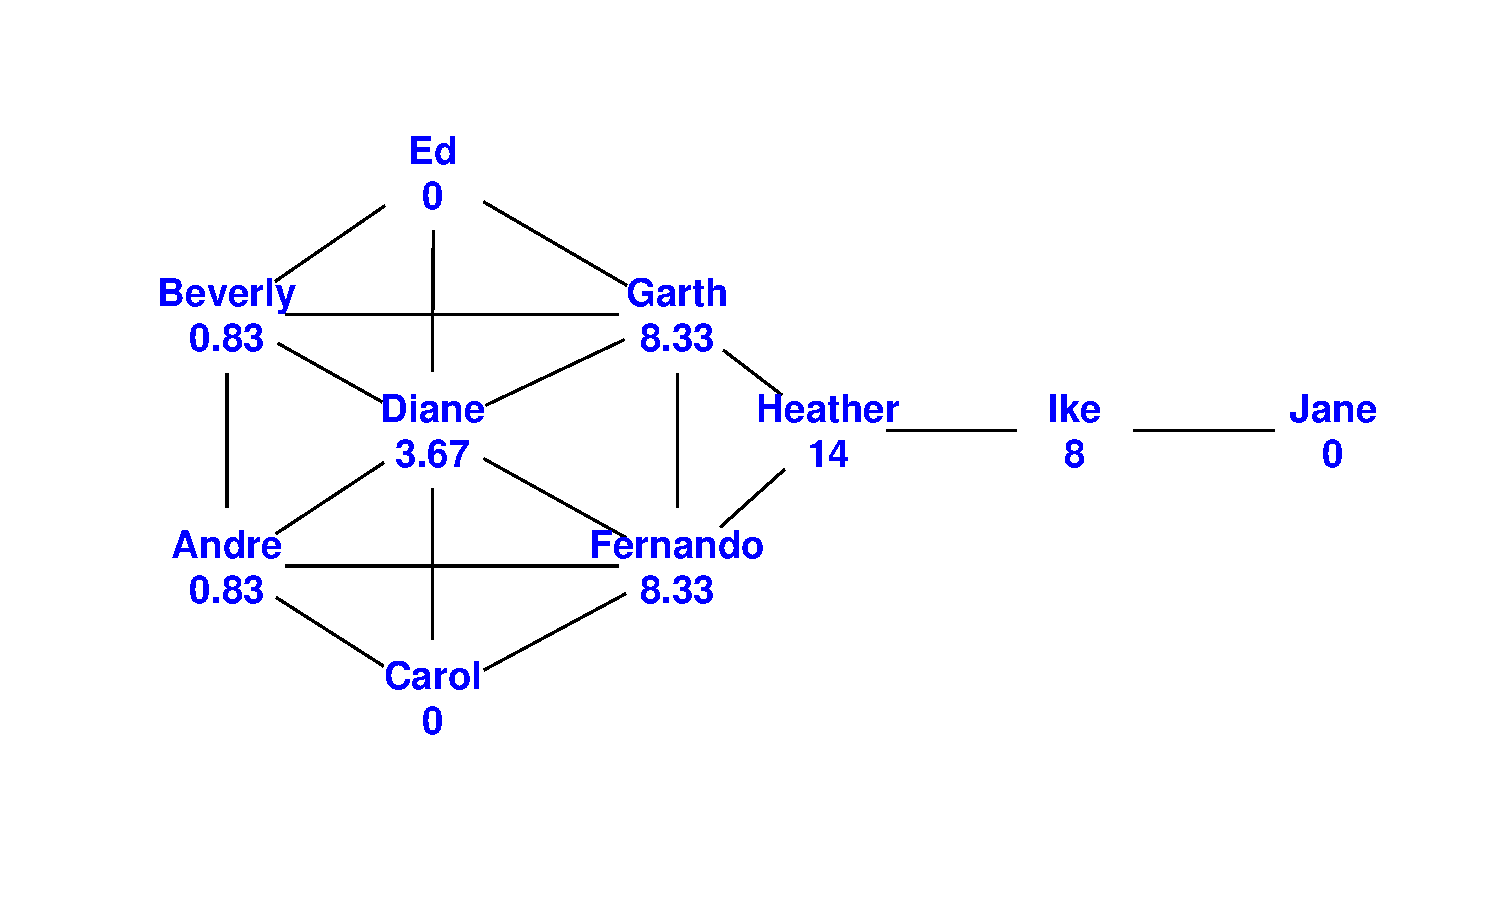
\includegraphics[width=0.8\textwidth]{centnet-betweenness}
\par Number of shortest paths going through a vertex.
\end{center}

\newpage
\stitle{Centrality, eigenvector centrality}
\begin{center}
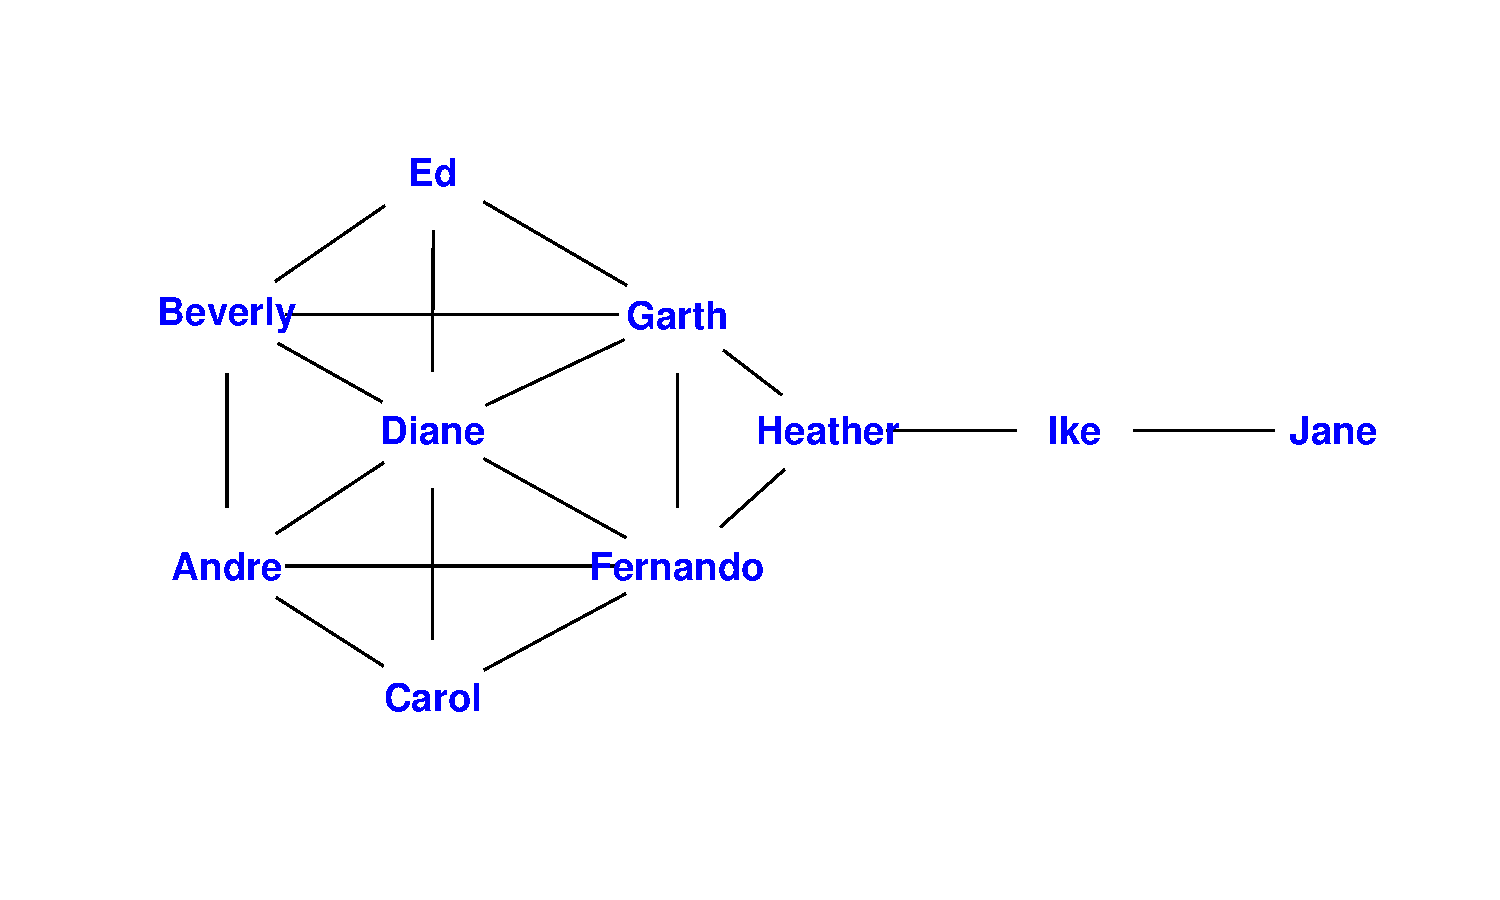
\includegraphics[width=0.8\textwidth]{centnet}
\par Number of adjacent edges, weighted by their ``goodness''.
\end{center}

\newpage
\stitle{Centrality, eigenvector centrality}
\begin{center}
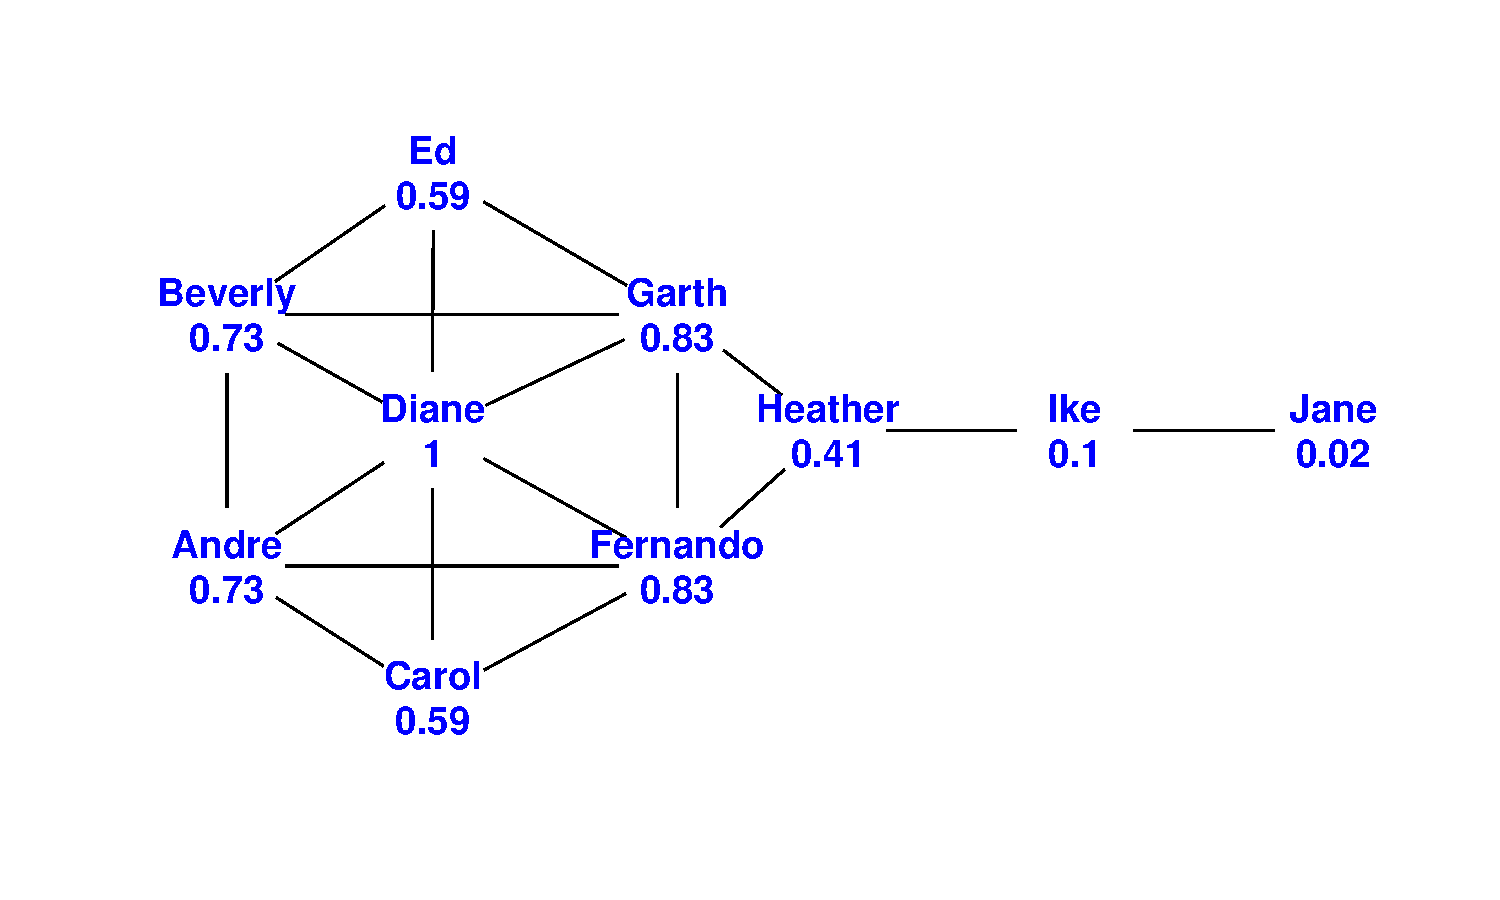
\includegraphics[width=0.8\textwidth]{centnet-evcent}
\par Number of adjacent edges, weighted by their ``goodness''.
\end{center}

\newpage
\stitle{Centrality, Burt's constraint}
\begin{center}
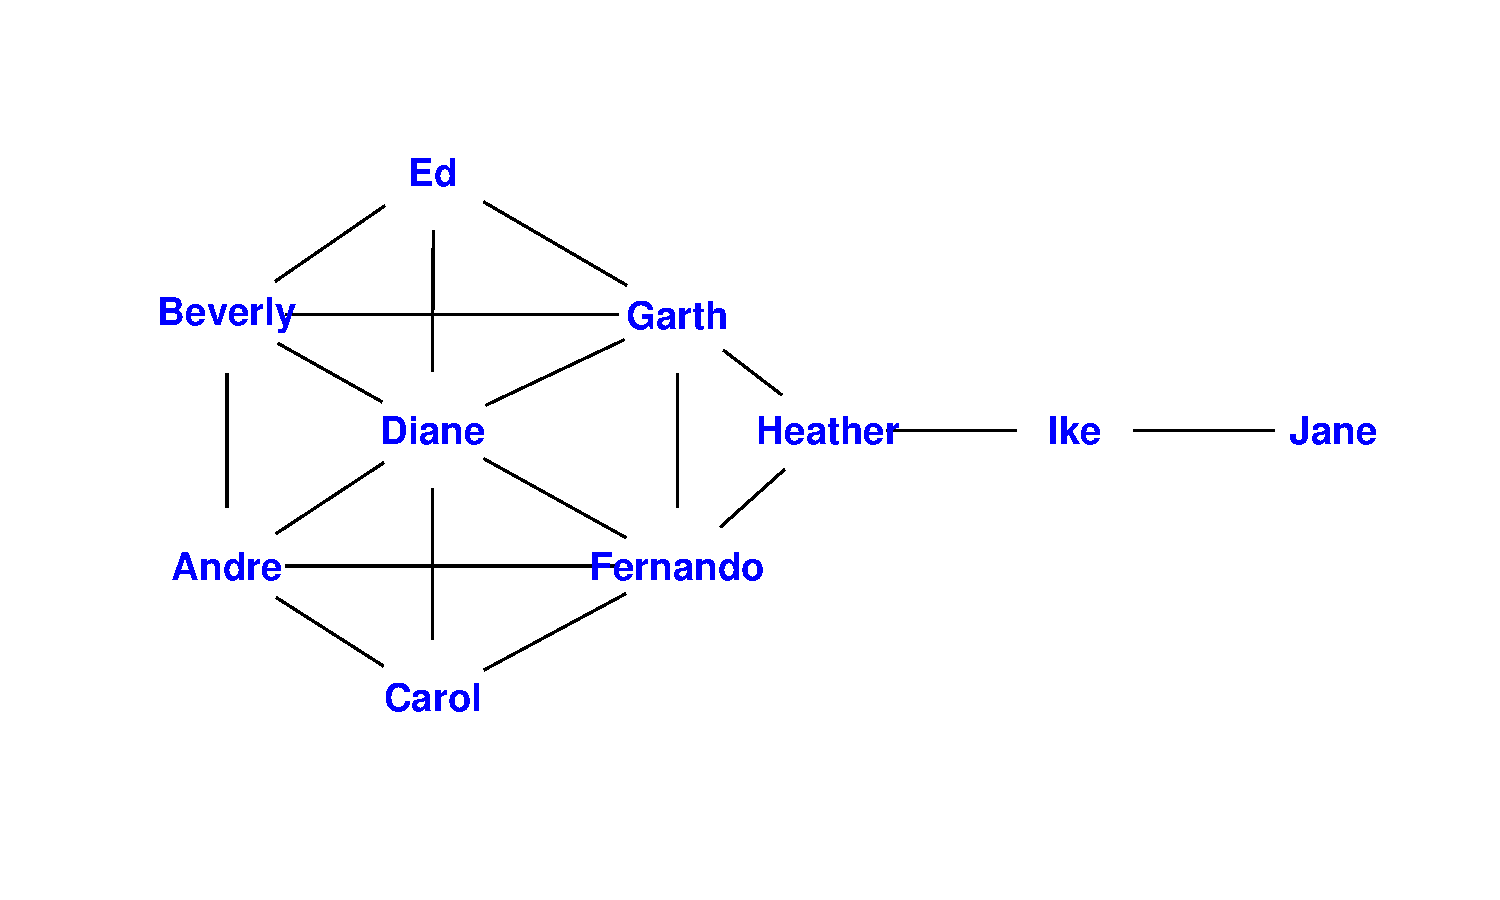
\includegraphics[width=0.8\textwidth]{centnet}
\par Benefit of brokering between other actors.
\end{center}

\newpage
\stitle{Centrality, Burt's constraint}
\begin{center}
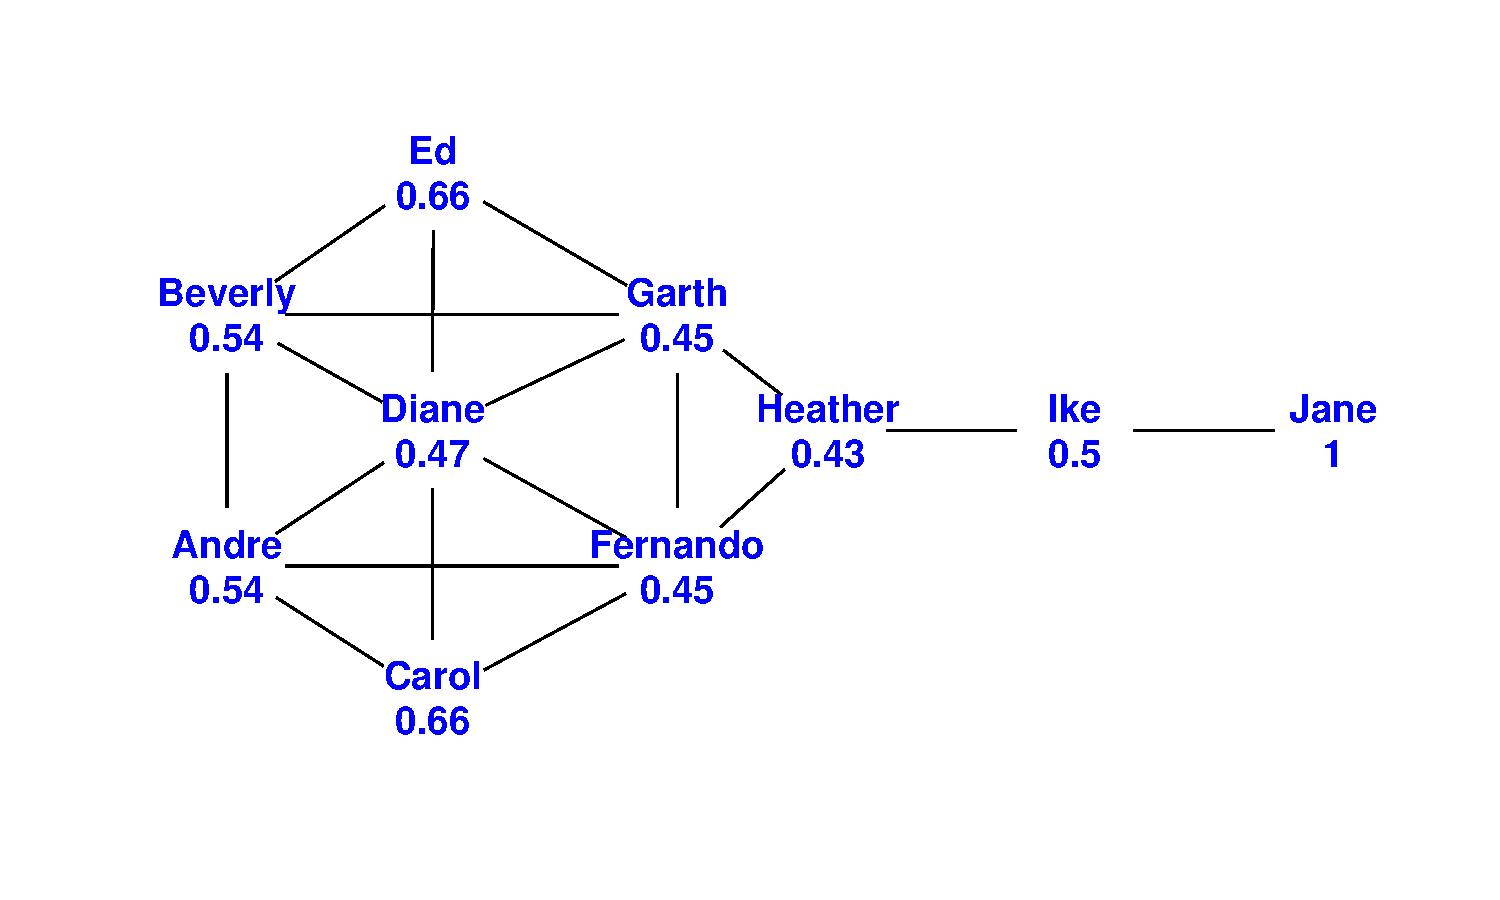
\includegraphics[width=0.8\textwidth]{centnet-constraint}
\par Benefit of brokering between other actors.
\end{center}

% \newpage
% \stitle{Centrality, information centrality}
% \begin{center}
% 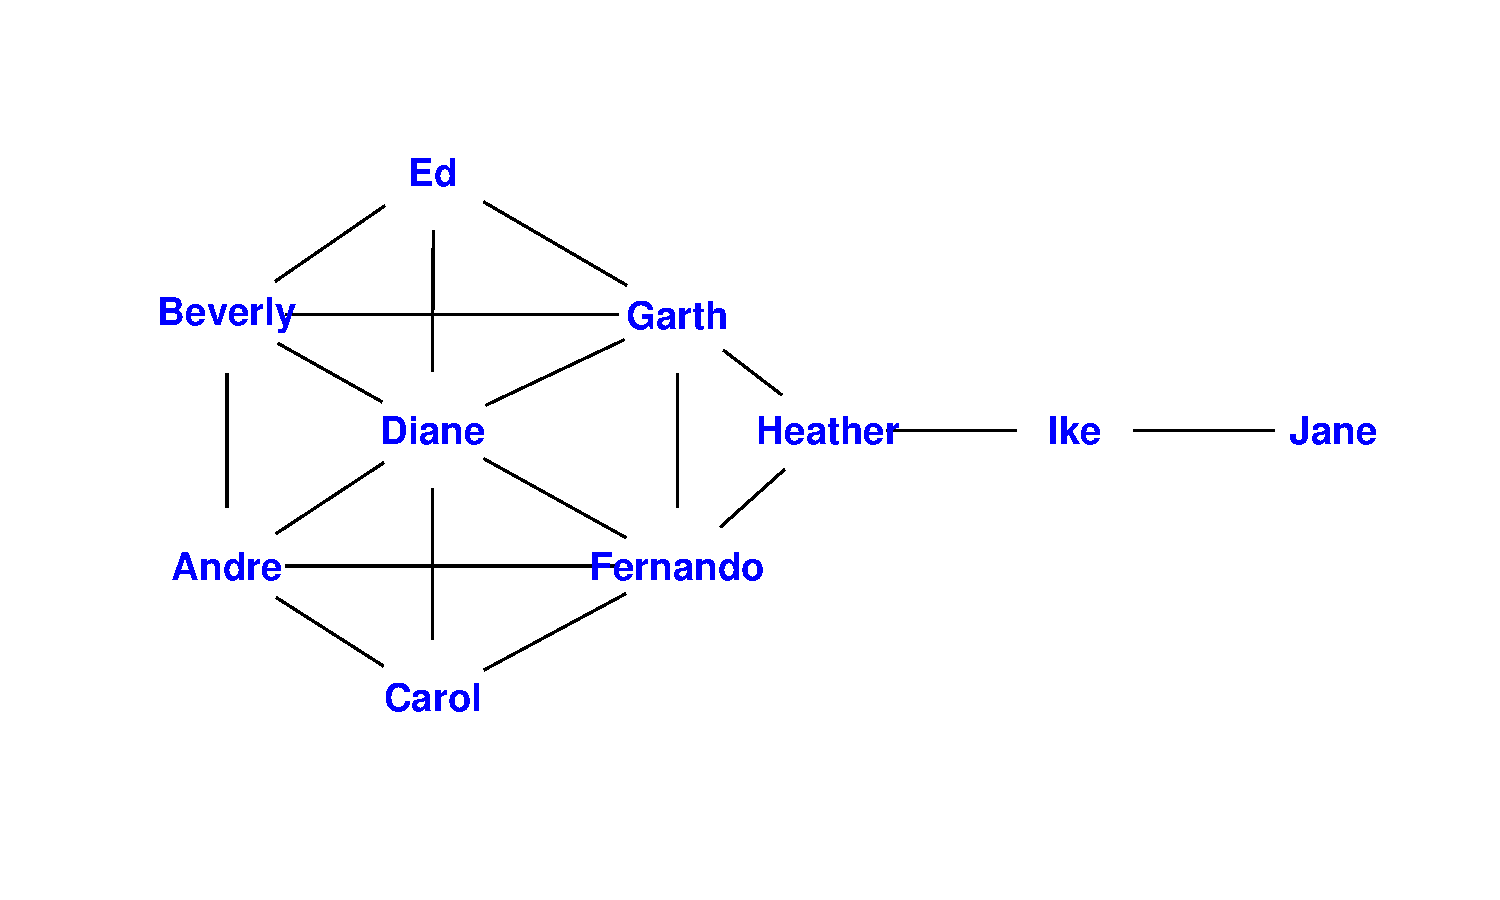
\includegraphics[width=0.8\textwidth]{centnet}
% \end{center}

% \newpage
% \stitle{Centrality, information centrality}
% \begin{center}
% 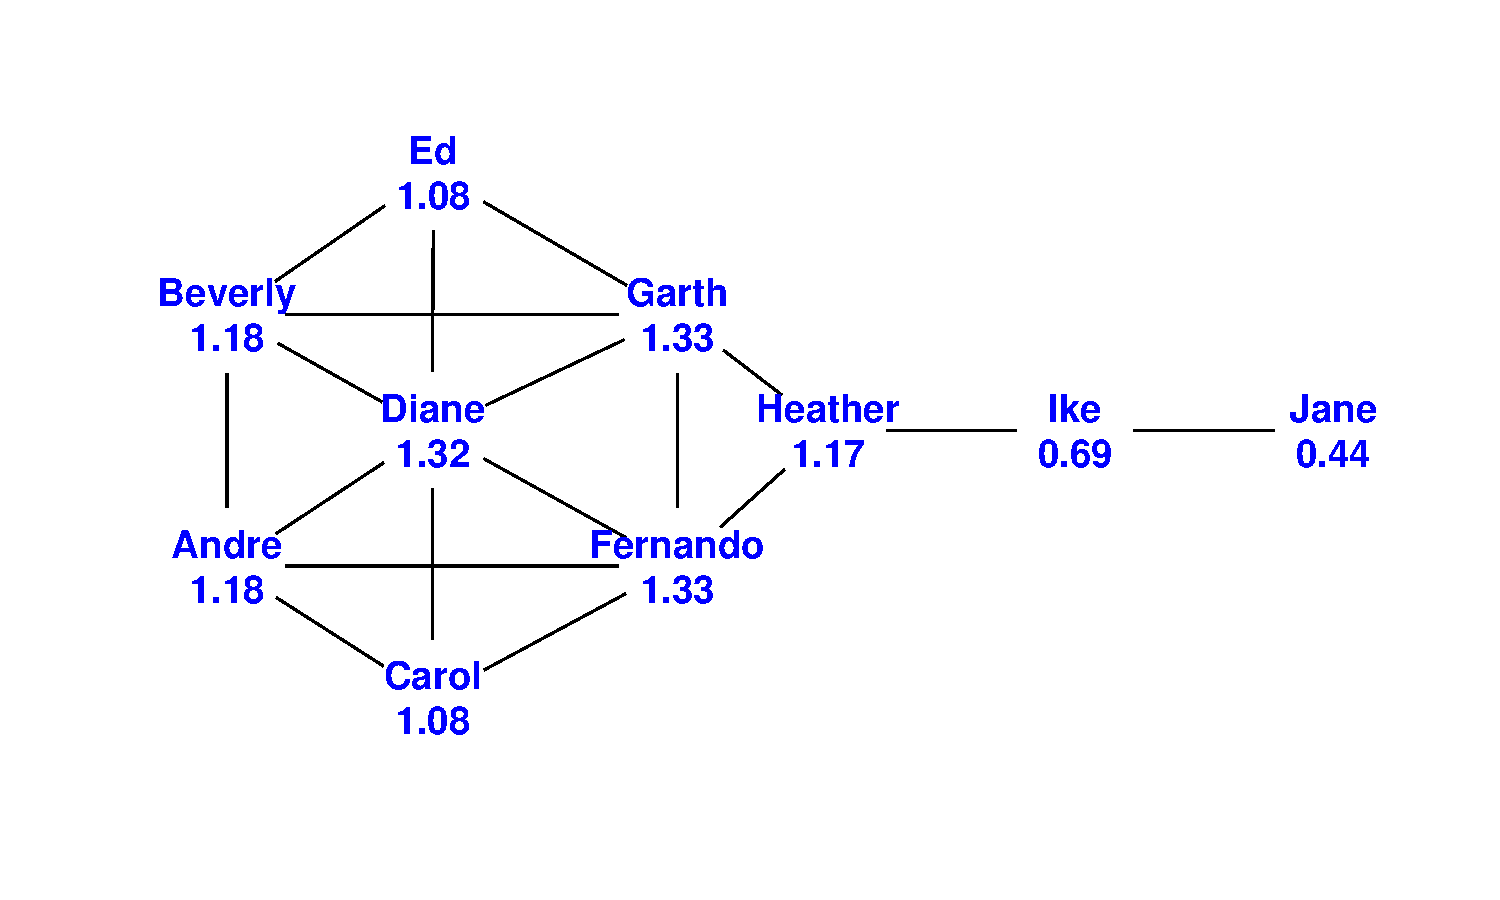
\includegraphics[width=0.8\textwidth]{centnet-infocent}
% \end{center}

\newpage
\stitle{Centrality, transitivity}
\begin{center}
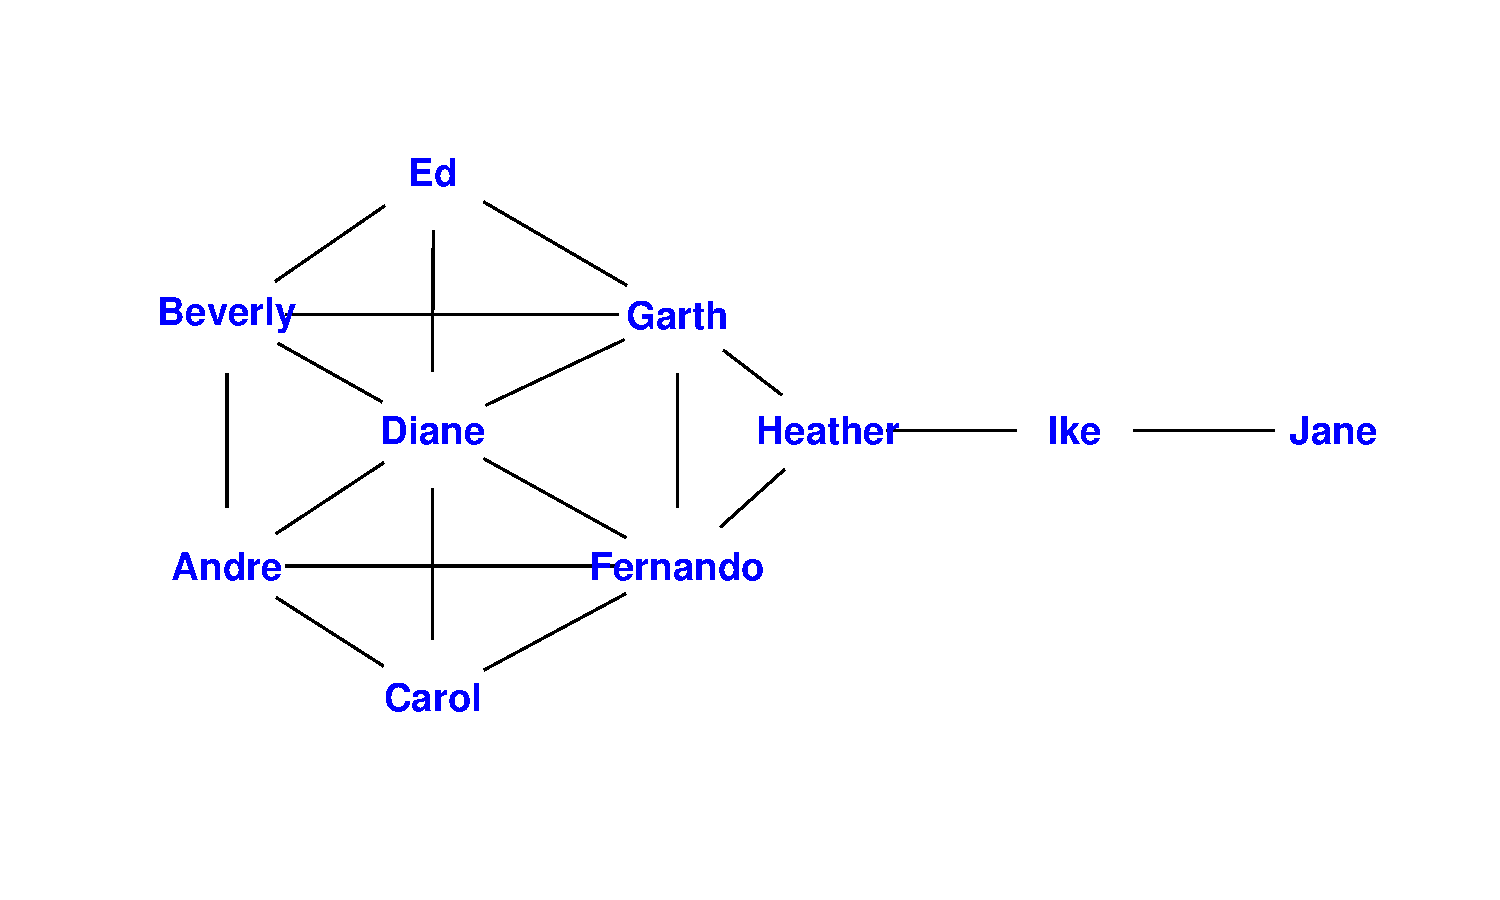
\includegraphics[width=0.8\textwidth]{centnet}
\par Are my friends also friends of each other?
\end{center}

\newpage
\stitle{Centrality, transitivity}
\begin{center}
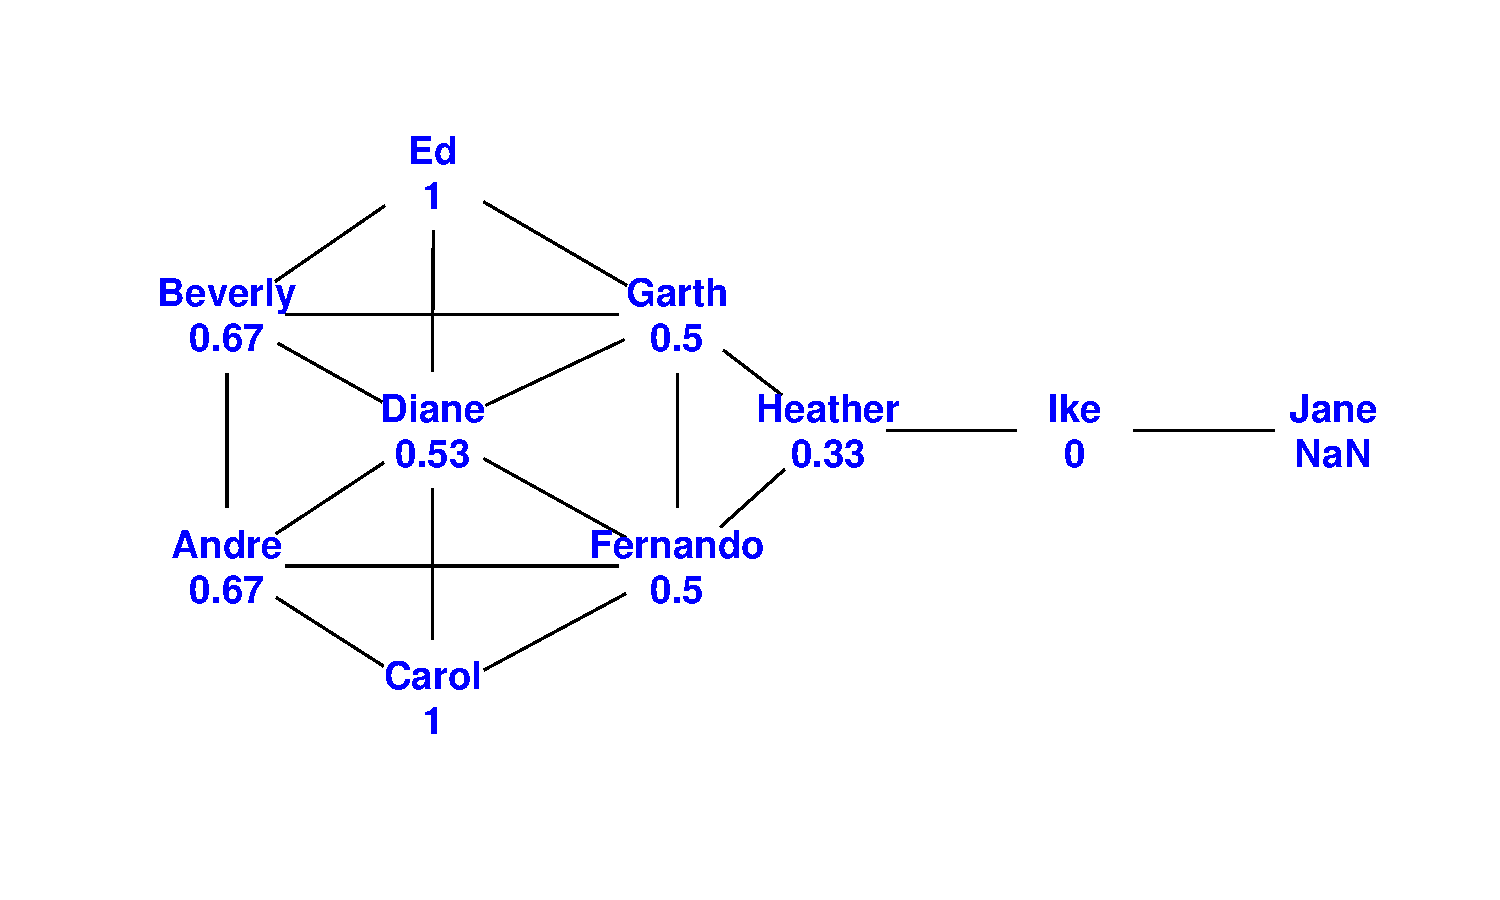
\includegraphics[width=0.8\textwidth]{centnet-trans}
\par Are my friends also friends of each other?
\end{center}

\newpage
\stitle{Sensitivity of centrality measures}
\begin{center}
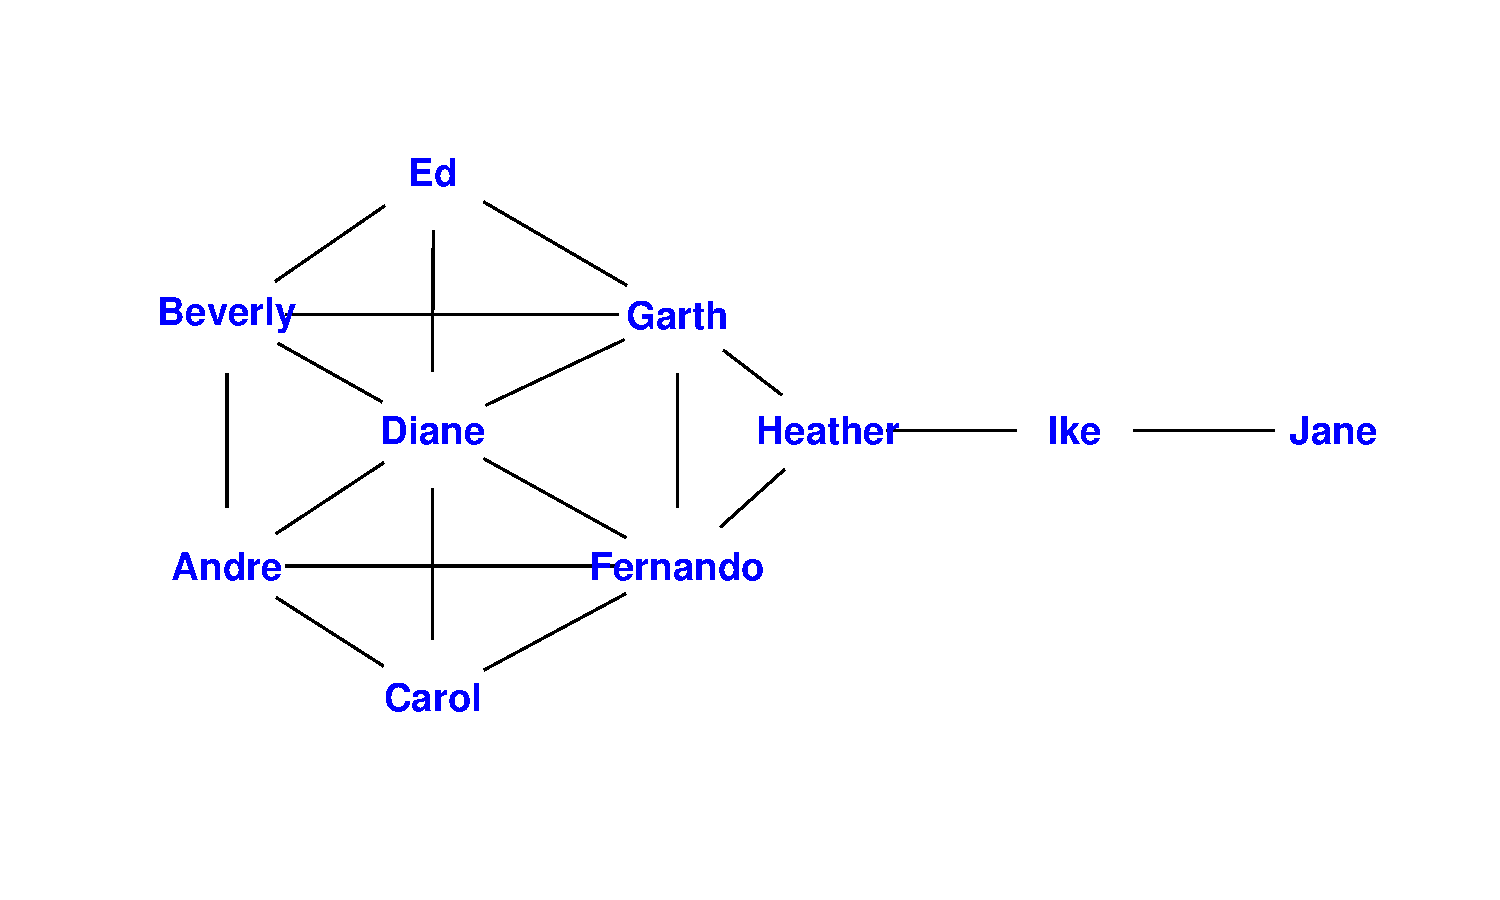
\includegraphics[width=0.8\textwidth]{centnet}
\par Remove two random edges, add two random edges.
\end{center}

\newpage
\stitle{Sensitivity of centrality measures}
\begin{narrow}{0cm}{15cm}
\begin{Myverb}
  cl <- numeric()
  for (i in 1:100) \{ 
    g2 <- delete.edges(g, sample(ecount(g), 2)-1)
    g2 <- g2 %u% 
  \item
    g\_nm(vcount(g), 2)
    cl <- cbind(cl, betweenness(g2))
  \}
  cl <- as.data.frame(t(cl))
  colnames(cl) <- V(g)$name  # $
  boxplot(cl, main="Sensitivity of betweenness")
\end{Myverb}
\end{narrow}

\newpage
\stitle{Sensitivity of centrality measures}
\begin{center}
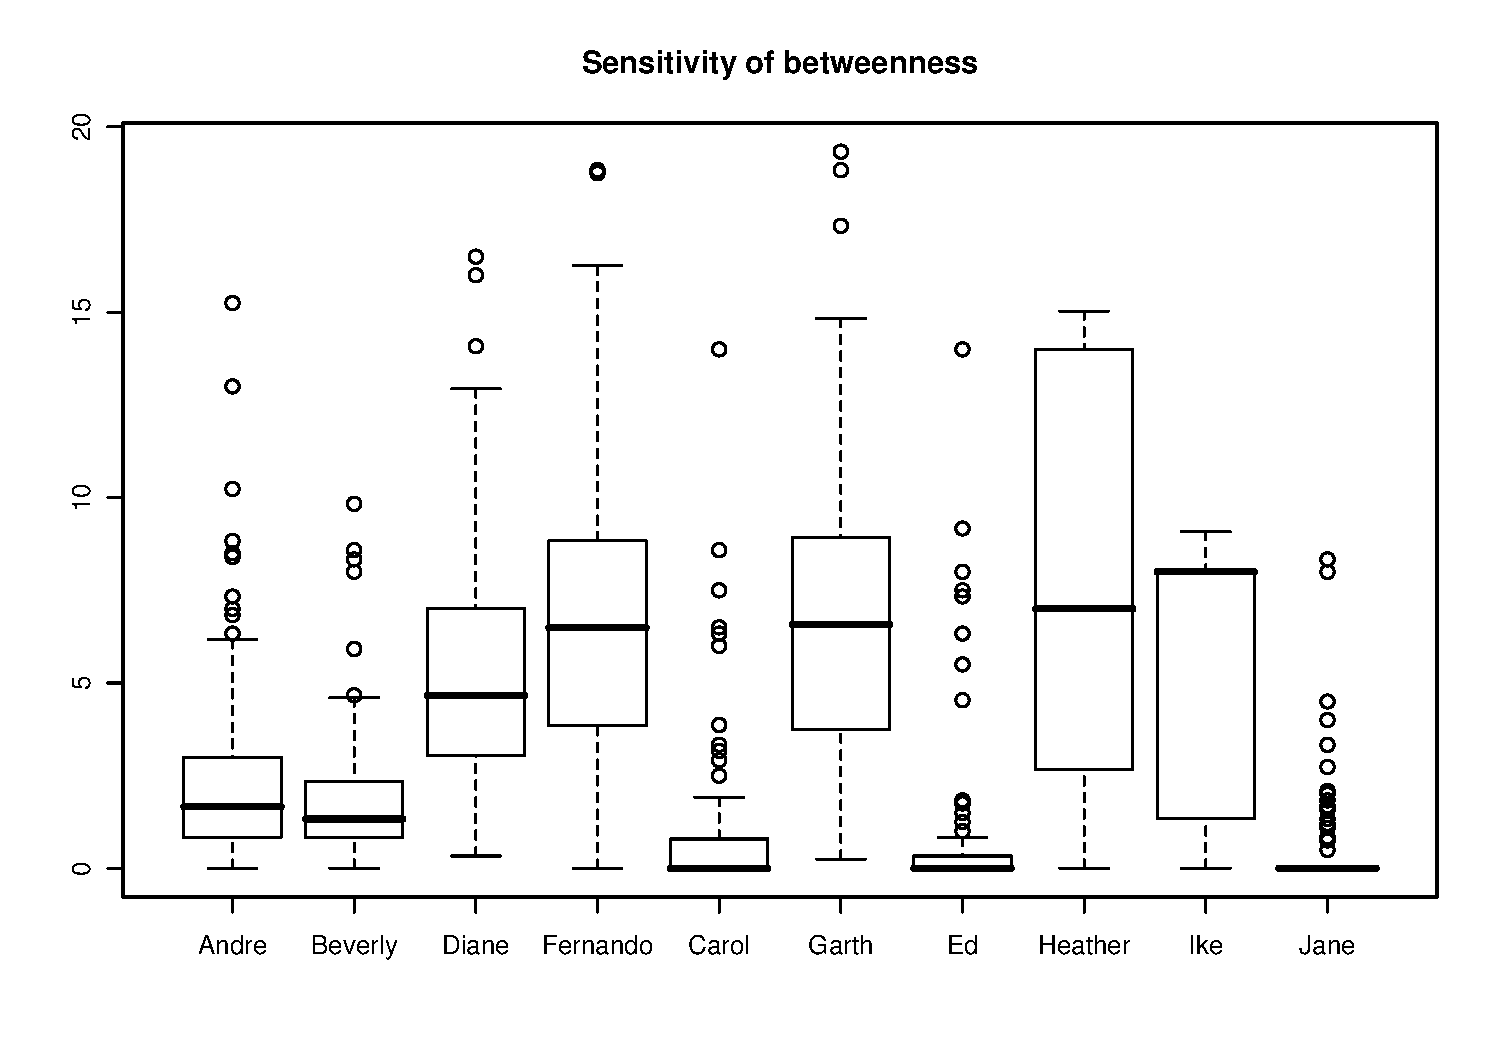
\includegraphics[width=0.8\textwidth]{boxplot}
\end{center}

\newpage
\stitle{Working with a (moderately) large graph}
\begin{Myverb}
  library(igraph)
  
  ## Load the jurisdiction network
  load("judicial.Rdata.gz")
  
  ## If we don't have it then create it again
  if (!exists("jg")) \{
    source("http://cneurocvs.rmki.kfki.hu/igraph/plus.R")
    vertices <- read.csv("http://cneurocvs.rmki.kfki.hu/igraph/judicial.csv")
    edges <- read.table("http://cneurocvs.rmki.kfki.hu/igraph/allcites.txt")
    jg <- graph.data.frame(edges, vertices=vertices, dir=TRUE)
  \}
  
  ## Basic data
  summary(jg)
  
  ## Is it a simple graph?
  is.simple(jg)
\end{Myverb}  

\newpage
\stitle{Working with a (moderately) large graph}
\begin{Myverb}
  ## Is it connected?
  is.connected(jg)
  
  ## How many components?
  no.clusters(jg)

  ## How big are these?
  table(clusters(jg)$csize)   #$
  
  ## In-degree distribution
  plot(degree.distribution(jg, mode="in"), log="xy")
  
  ## Out-degree distribution
  plot(degree.distribution(jg, mode="out"), log="xy")
  
  ## Largest in- and out-degree, total degree
  max(degree(jg, mode="in"))
  max(degree(jg, mode="out"))
  max(degree(jg, mode="all"))
\end{Myverb}  

\newpage
\stitle{Working with a (moderately) large graph}
\begin{Myverb}  
  ## Density
  graph.density(jg)
  
  ## Transitivity
  transitivity(jg)
  
  ## Transitivity of a random graph of the same size
  g <- erdos.renyi.game(vcount(jg), ecount(jg), type="gnm")
  transitivity(g)
  
  ## Dyad census
  dyad.census(jg)
  
  ## Triad census
  triad.census(jg)
  \end{Myverb}  

\newpage
\stitle{Working with a (moderately) large graph}
\begin{Myverb}  
  ## Authority and Hub scores
  authority.score(jg)$vector
  cor(authority.score(jg)$vector, V(jg)$auth)
  
  hub.score(jg)$vector
  cor(hub.score(jg)$vector, V(jg)$hub)
\end{Myverb} 

\newpage
\stitle{Big table of ``what can be run''}

\renewcommand{\arraystretch}{1.7}
\begin{tabularx}{\textwidth}{l|X}
Fast (millions) & creating graphs (most of the time) \bull
       structural modification (add/delete edges/vertices) \bull 
       subgraph \bull simplify \bull graph.decompose \bull 
       degree \bull clusters \bull graph.density \bull is.simple,
       is.loop, is.multiple \bull articulation points and biconnected
       components \bull ARPACK stuff: page.rank, hub.score,
       authority.score, evcent \bull transitivity \bull Burt's
       constraint \bull dyad \& triad census, graph motifs \bull
       $k$-cores \bull MST \bull reciprocity \bull modularity \bull
       closeness and (edge) betweenness \it{estimation} \bull shortest
       paths from one source \bull generating $G_{n,p}$ and $G_{n,m}$
       graphs \bull generating PA graphs with various PA exponents
       \bull topological sort \\
\hline
Slow (10000) & closeness \bull diameter \bull betweenness \bull all-pairs
       shortest paths, average path length \bull most layout
       generators \bull \\
\hline
Very slow (100) & cliques \bull cohesive blocks \bull edge/vertex
            connectivity \bull maximum flows and minimum cuts \bull 
            bonpow \bull alpha centrality \bull (sub)graph isomorphism\\
\end{tabularx}

\newpage
\stitle{Why is igraph sooooo slow?}

\begin{tabularx}{\textwidth}{X|l}
cliques and independent vertex sets & Hard problem \\
\hline
cohesive blocks                     & Semi-hard problem \\
\hline
edge/vertex connectivity, maximum flows and minimum cuts & Semi-hard
                                      problem \\
\hline
Bonacich's power centrality, alpha centrality & Poor implementation \\
\hline
(sub)graph isomorphism & Hard problem \\
\hline
\emph{anything else} & \emph{contact us if you want to speed it up} \\
\end{tabularx}

% \newpage
% \stitle{Generating random graphs}
%% TODO

\newpage
\stitle{Connection to other network/graph software}
\begin{itemize}
\item \texttt{sna} and \texttt{network} R packages. Currently throught
  adjacency matrices. Use namespaces!\pause
\item Pajek. \texttt{.net} file format is supported. \pause
\begin{Myverb}
  g <- read.graph("http://vlado.fmf.uni-lj.si/pub/networks/data/", 
       format="pajek")
\end{Myverb}
\pause
\item Visone. Use GraphML format. \pause
\item Cytoscape. Use GML format. \pause
\item GraphViz. igraph can write \texttt{.dot} files. \pause
\item In general. The \emph{GraphML} and \emph{GML} file formats 
  are fully supported, many programs can read/write these.
\end{itemize}

\newpage
\stitle{Community structure detection}
\begin{center}
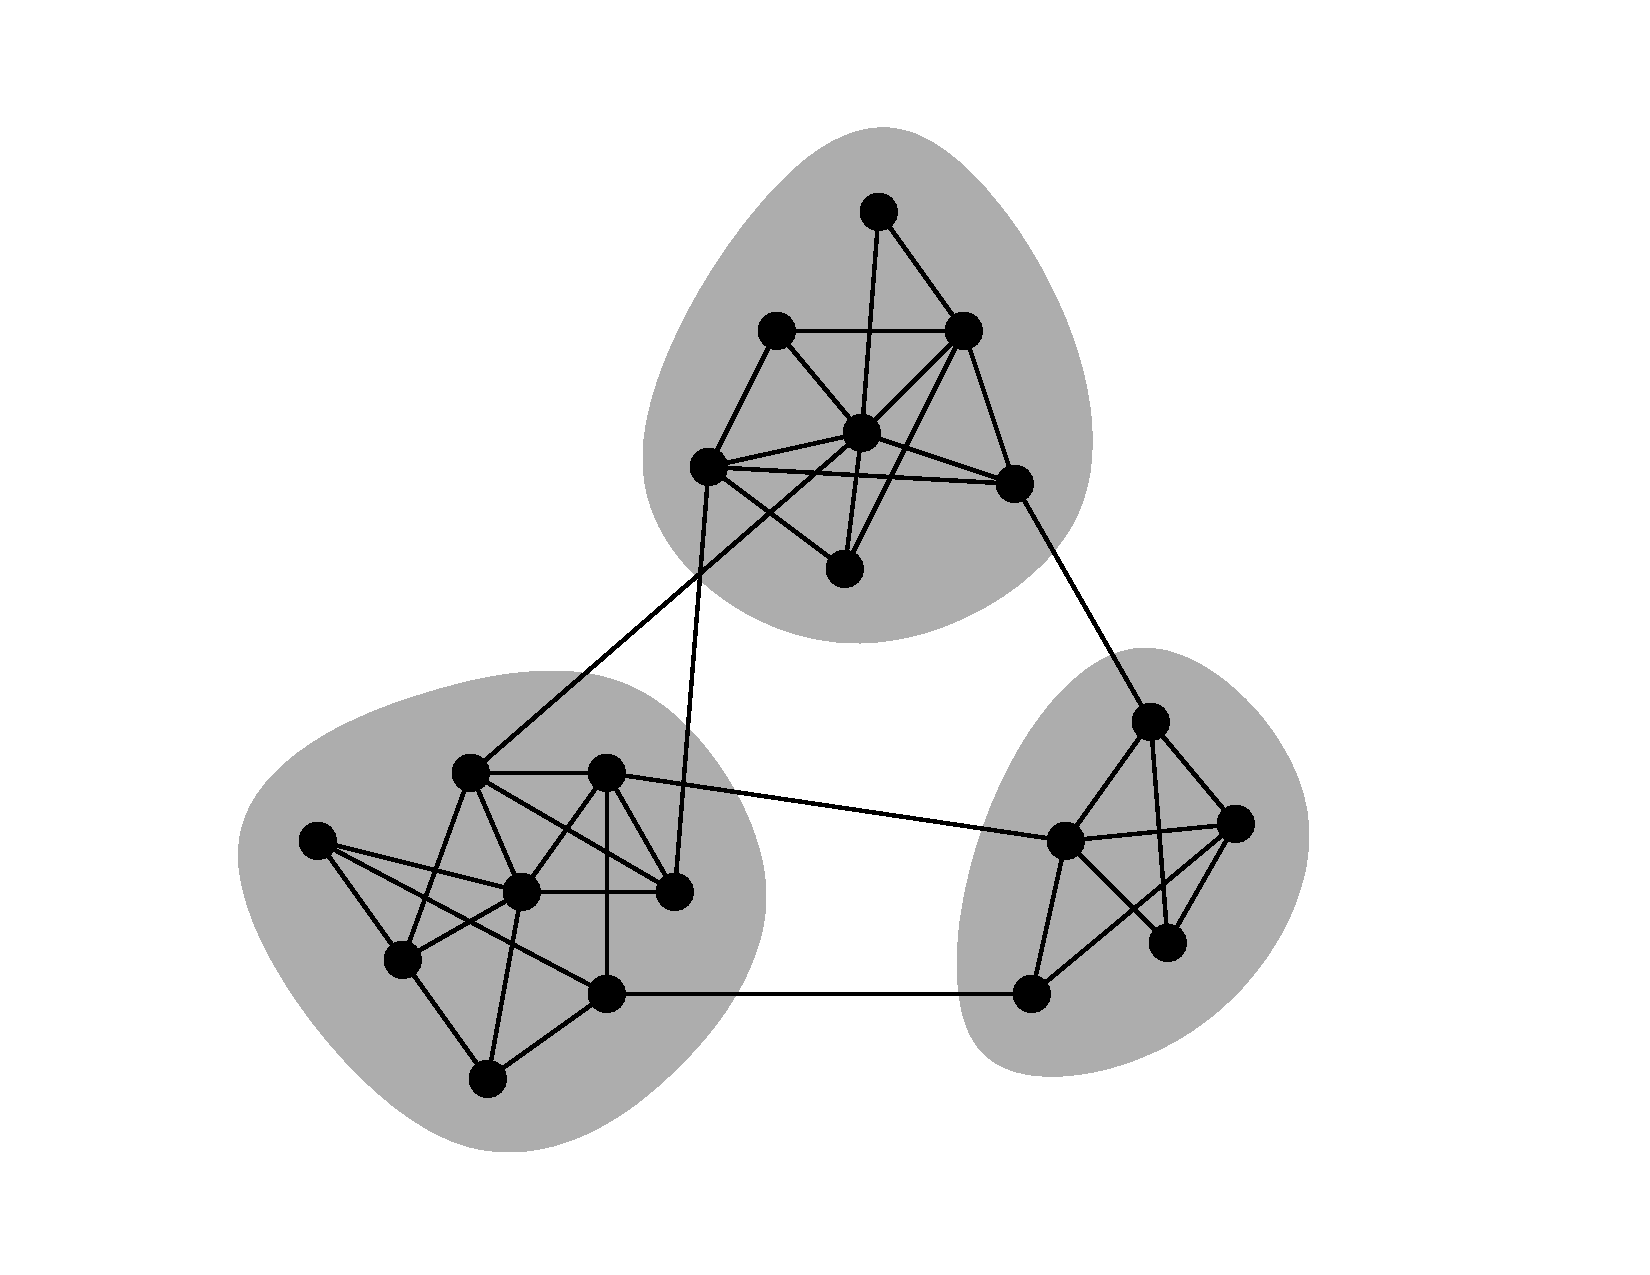
\includegraphics[width=0.7\textwidth]{communities}\\
\small(Modularity and community structure in networks, by Mark Newman,
2006)
\end{center}

\newpage
\stitle{Modularity score}
\begin{narrow}{0cm}{15cm}
\begin{itemize}
\item How to define what is modular? Many proposed definitions, here
  is a popular one:
  \[ Q = \frac1{2|E|}\sum_{vw} [A_{vw} - p_{vw} ]\delta(c_v,c_w). \] \pause
\item Random graph null model: 
  \[ p_{vw} = p = \frac{1}{|V|(|V|-1)} \] \pause
\item Degree sequence based null model:
  \[ p_{vw} = \frac{k_vk_w}{2|E|} \]
\end{itemize}
\end{narrow}

\newpage
\stitle{``Fast-greedy'' algorithm}
\begin{center}
A Clauset, MEJ Newman, C Moore: Finding community structure in very
large networks, \url{http://www.arxiv.org/abs/cond-mat/0408187}\\
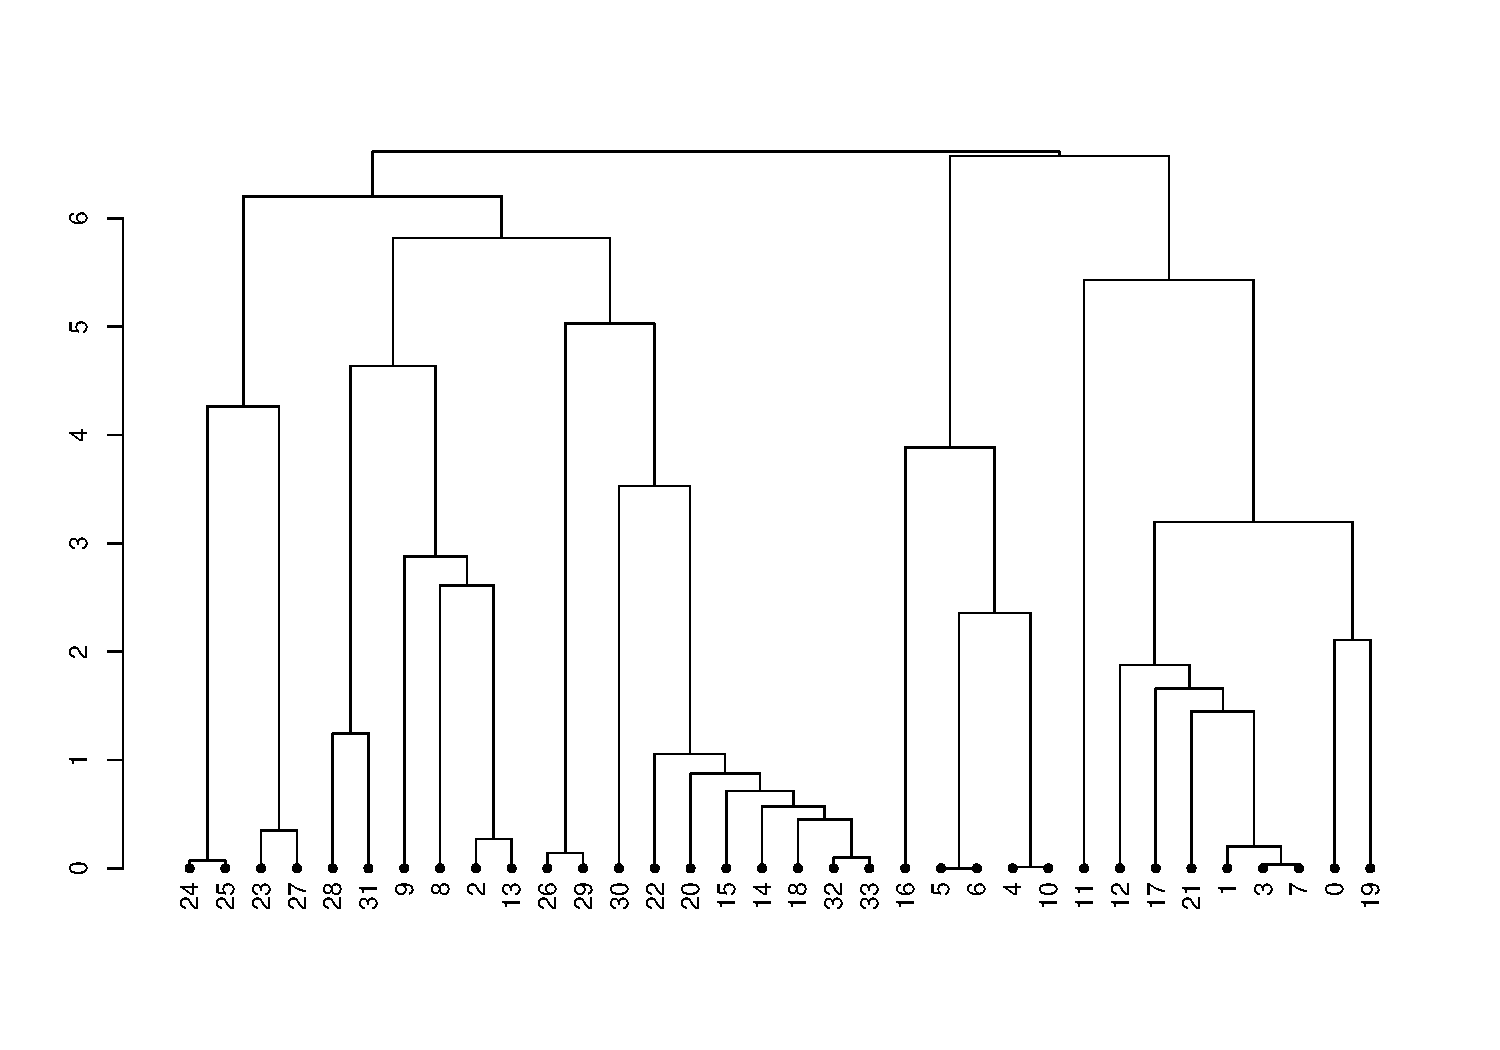
\includegraphics[width=0.75\textwidth]{dend}
\end{center}

\newpage
\stitle{``Spinglass'' algorithm}
\begin{center}
J. Reichardt and S. Bornholdt: Statistical Mechanics of Community
Detection, Phys. Rev. E, 74, 016110 (2006),
\url{http://arxiv.org/abs/cond-mat/0603718}
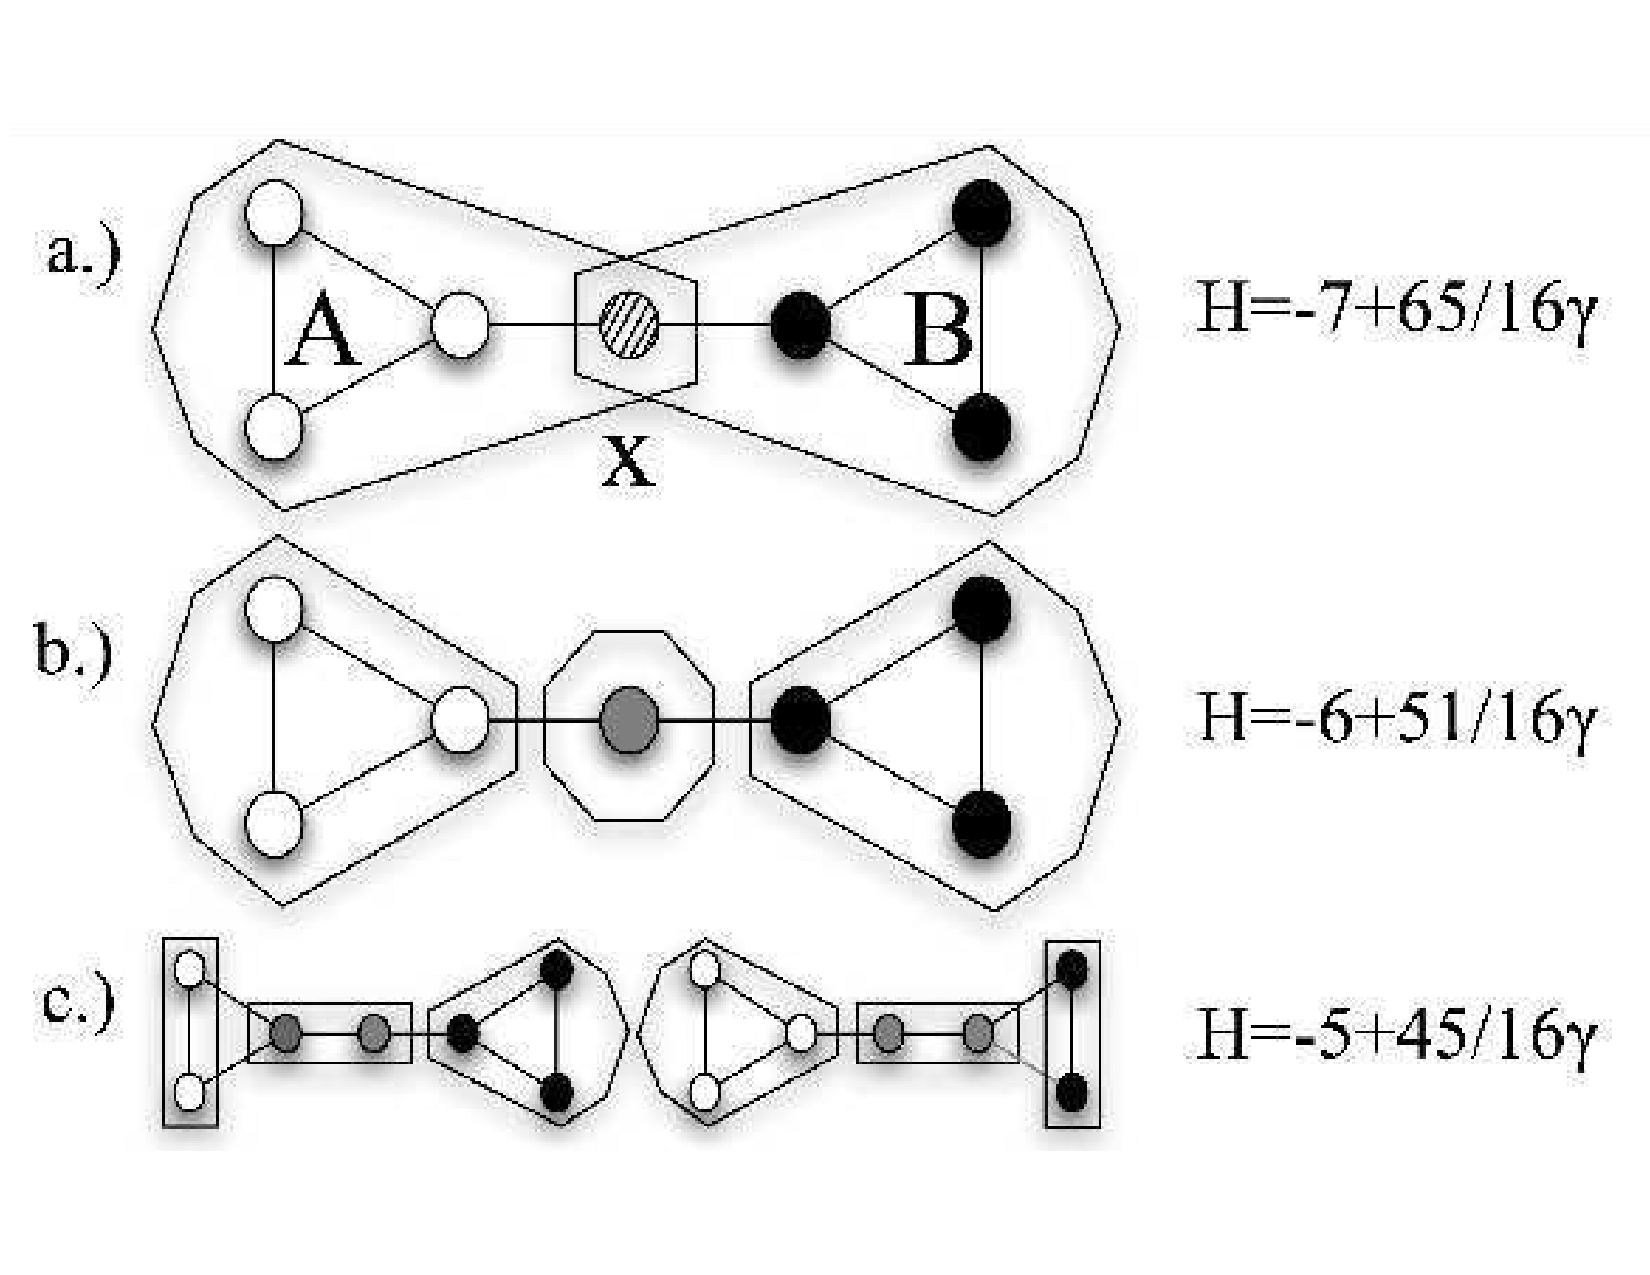
\includegraphics[width=0.42\textwidth]{spinglass1}\hfil%
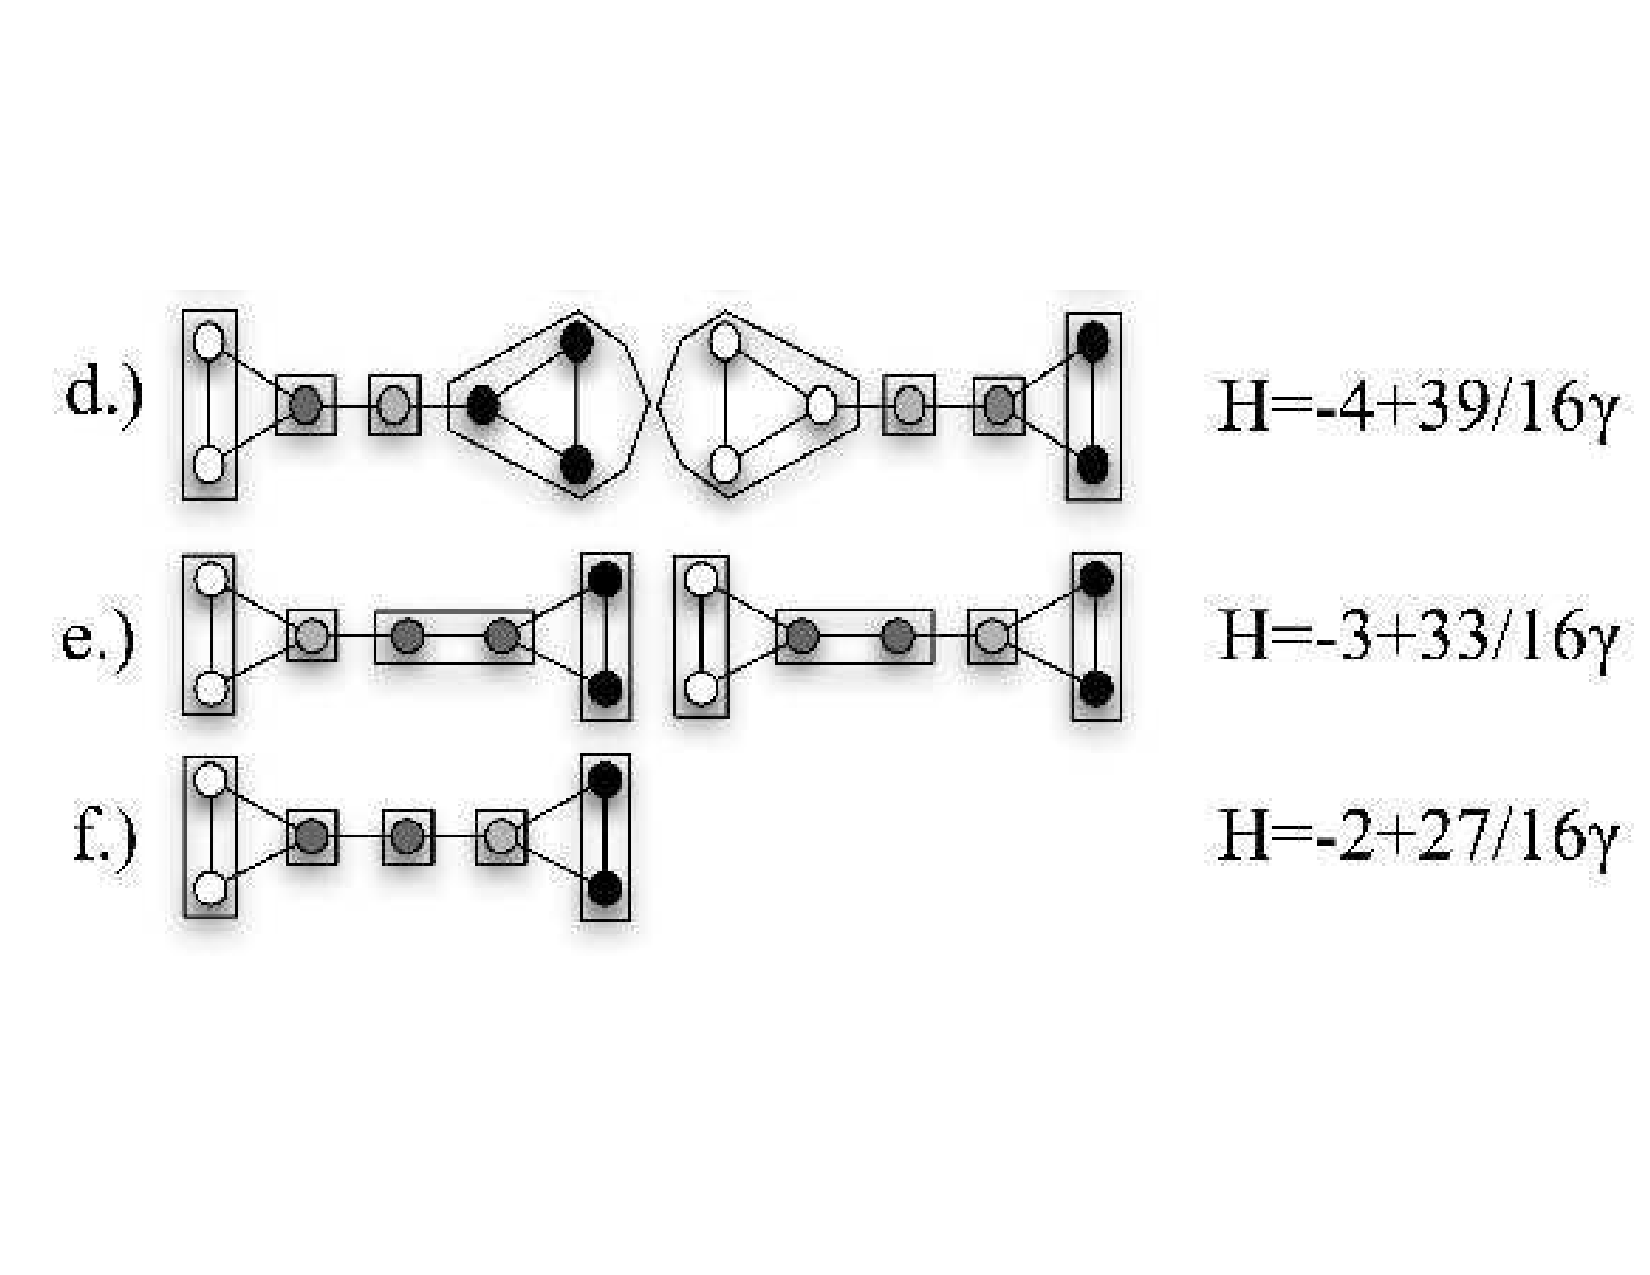
\includegraphics[width=0.42\textwidth]{spinglass2}
\end{center}

\newpage
\stitle{Cohesive blocks}

\begin{itemize}
\item `Structural Cohesion and Embeddedness: a Hierarchical
Concept of Social Groups' by J.Moody and D.White, Americal
Sociological Review, 68, 103--127, 2003 \pause
\item Definition 1: A collectivity is structurally cohesive to the extent
  that the social relations of its members hold it together.  \pause
\item Definition 2: A group is structurally cohesive to the extent that
  multiple independent relational paths among all pairs of members hold
  it together. \pause
\item Vertex-independent paths and vertex connectivity. \pause
\item Vertex connectivity and network flows.
\end{itemize}

\newpage
\stitle{Cohesive blocks}
\vspace*{-3cm}
{\centering
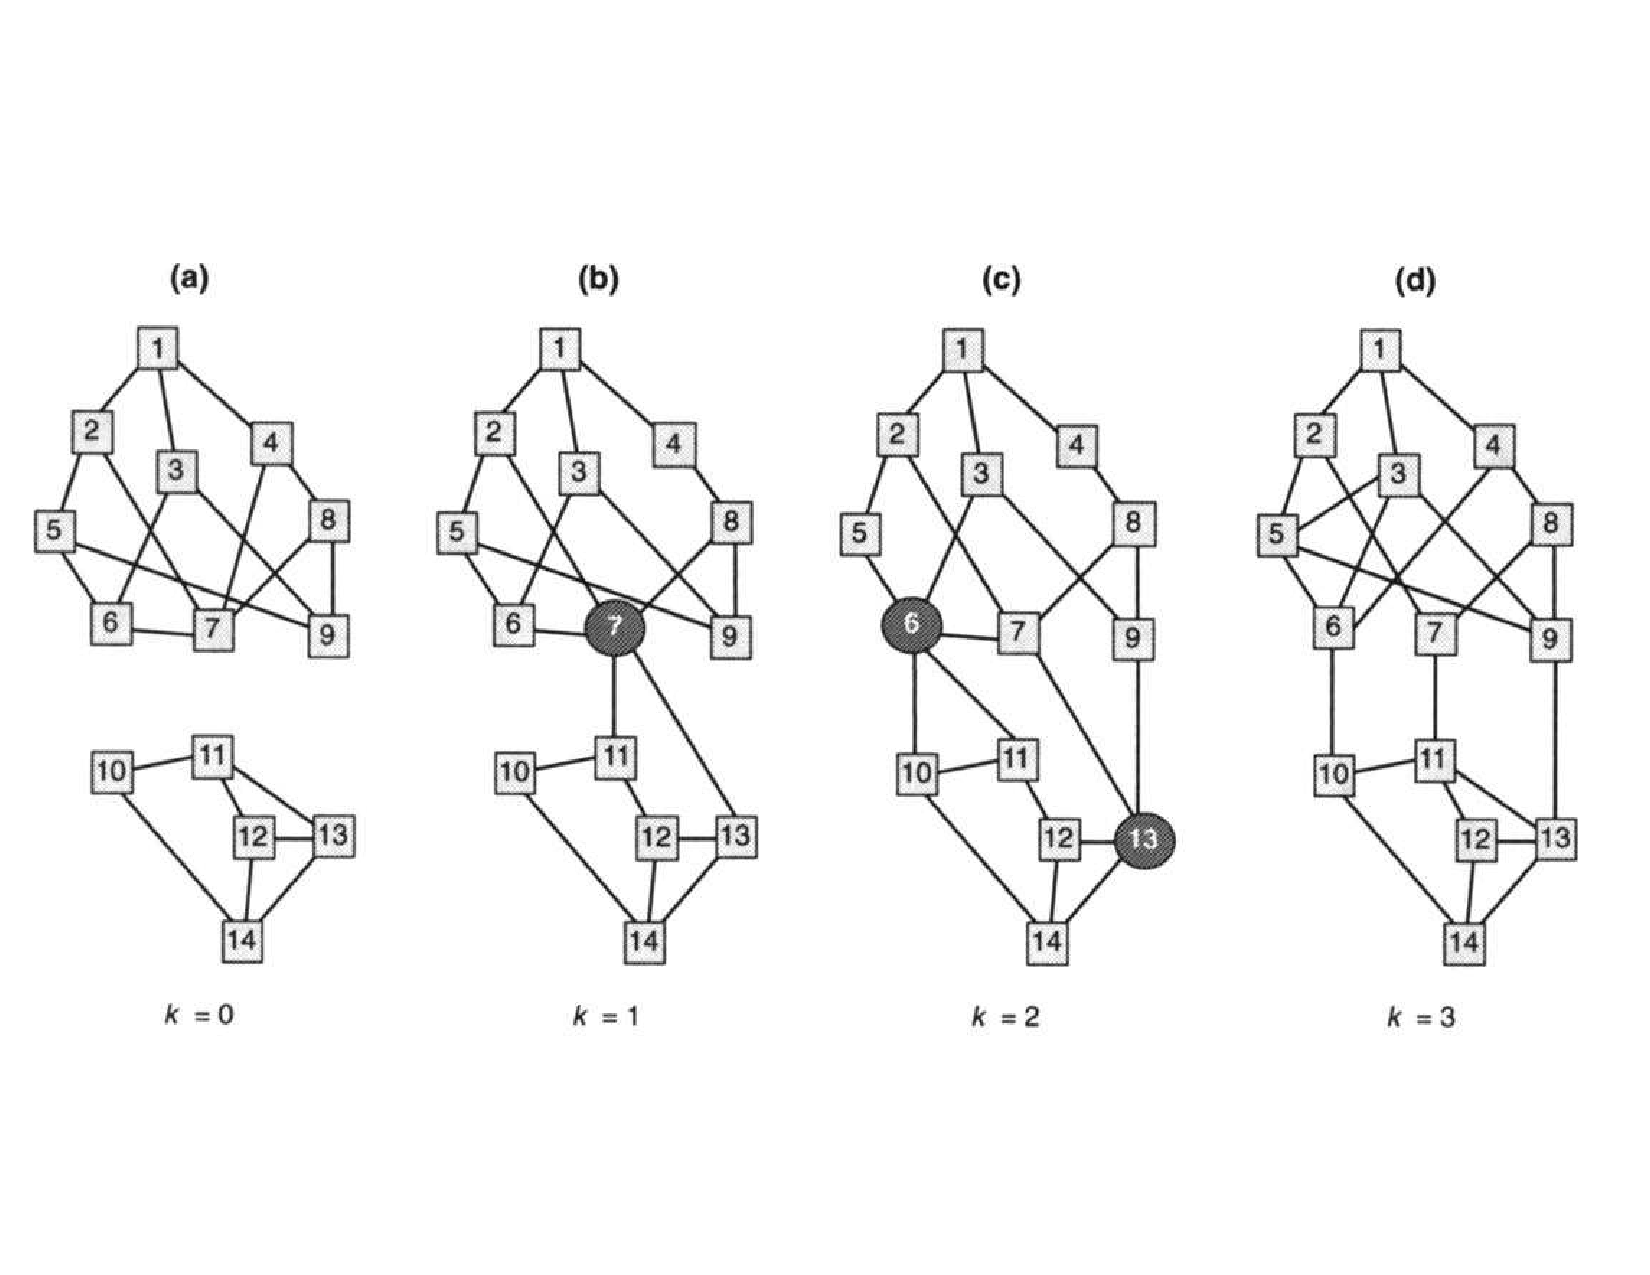
\includegraphics[width=0.9\textwidth]{../images/groups}\\
}

\newpage
\stitle{Cohesive blocks}
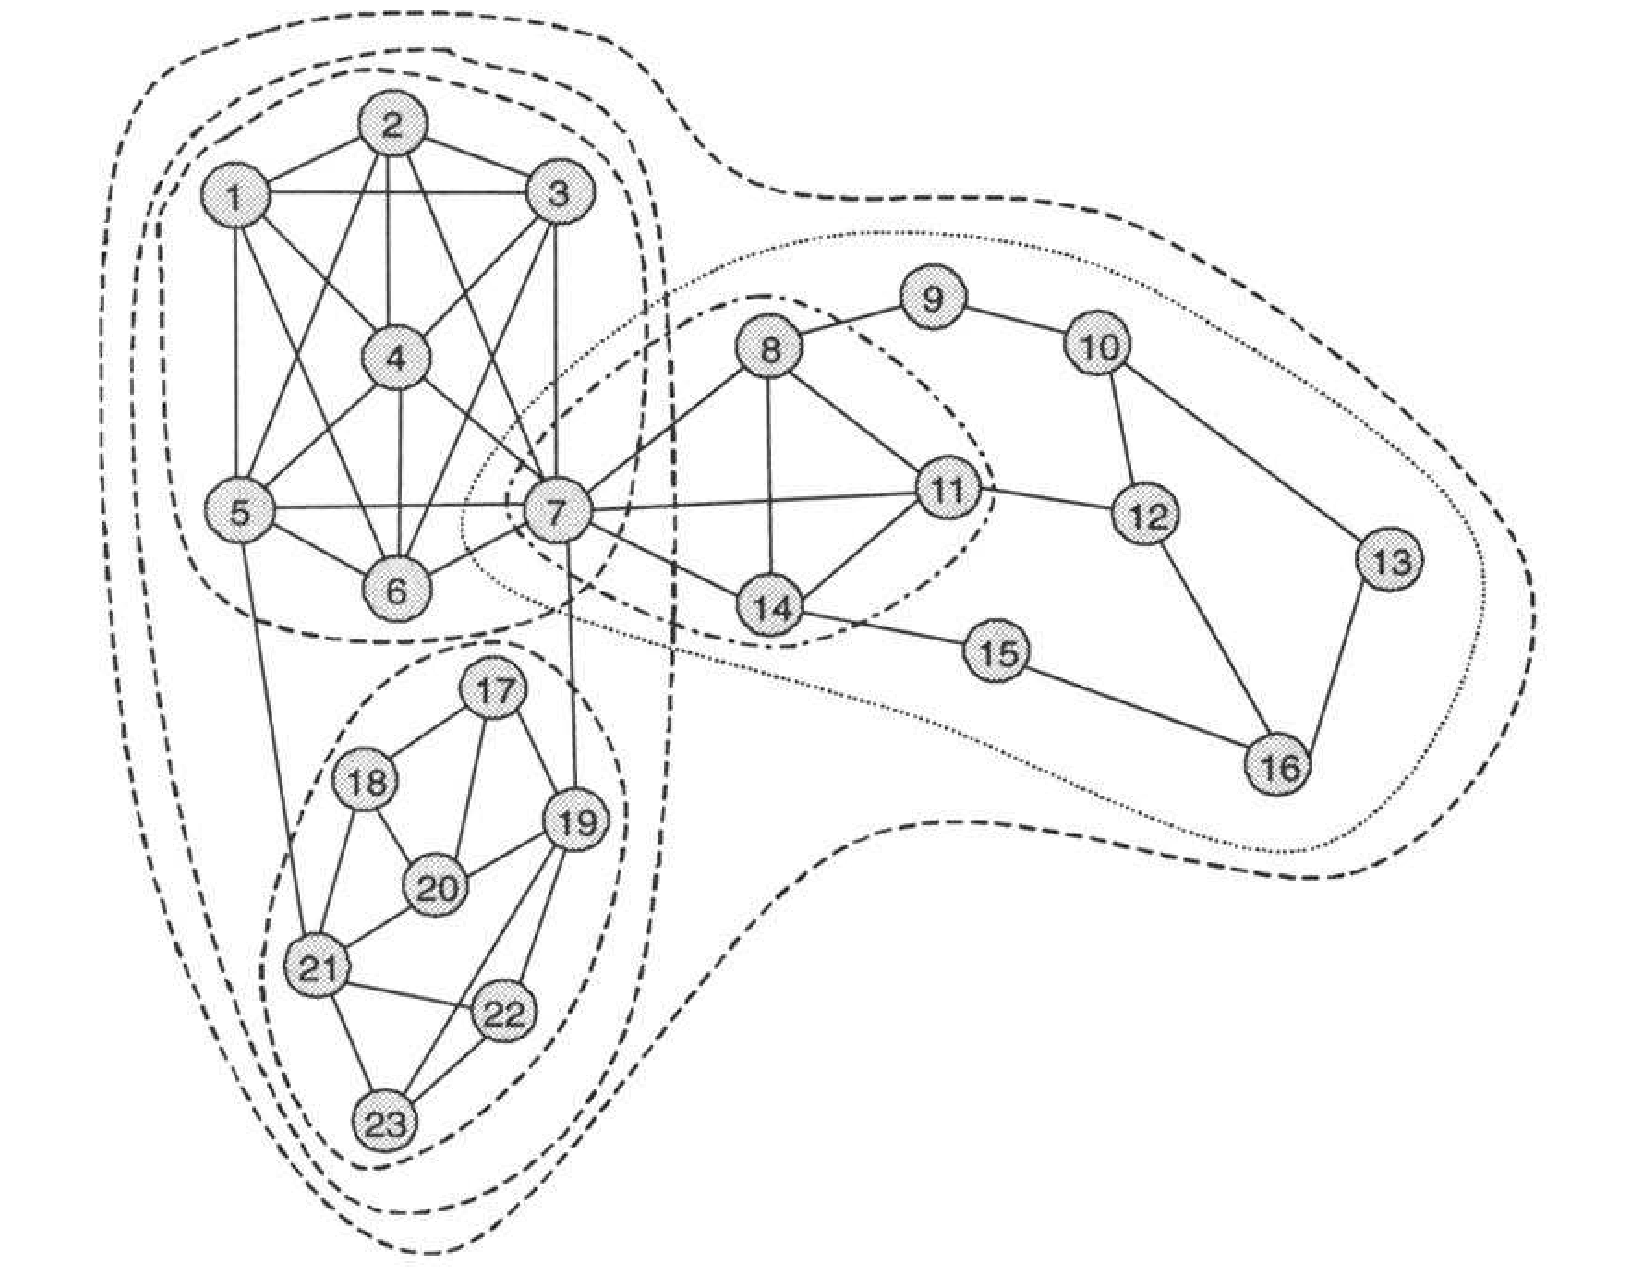
\includegraphics[width=0.6\textwidth]{../images/cblocks}\\

\newpage
\stitle{Cohesive blocks}
\begin{narrow}{0cm}{15cm}
\begin{Myverb}
  cb <- graph( c(1,2,1,3,1,4,1,5,1,6,
                2,3,2,4,2,5,2,7,
                3,4,3,6,3,7,
                4,5,4,6,4,7,
                5,6,5,7,5,21,
                6,7,
                7,8,7,11,7,14,7,19,
                8,9,8,11,8,14,
                9,10,
                10,12,10,13,
                11,12,11,14,
                12,16, 13,16, 14,15, 15,16,
                17,18,17,19,17,20,
                18,20,18,21,
                19,20,19,22,19,23,
                20,21, 21,22,21,23,
                22,23)-1, dir=FALSE)

  V(cb)$label <- seq(vcount(cb))  # $
\end{Myverb}
\end{narrow}

\newpage
\stitle{Cohesive blocks}
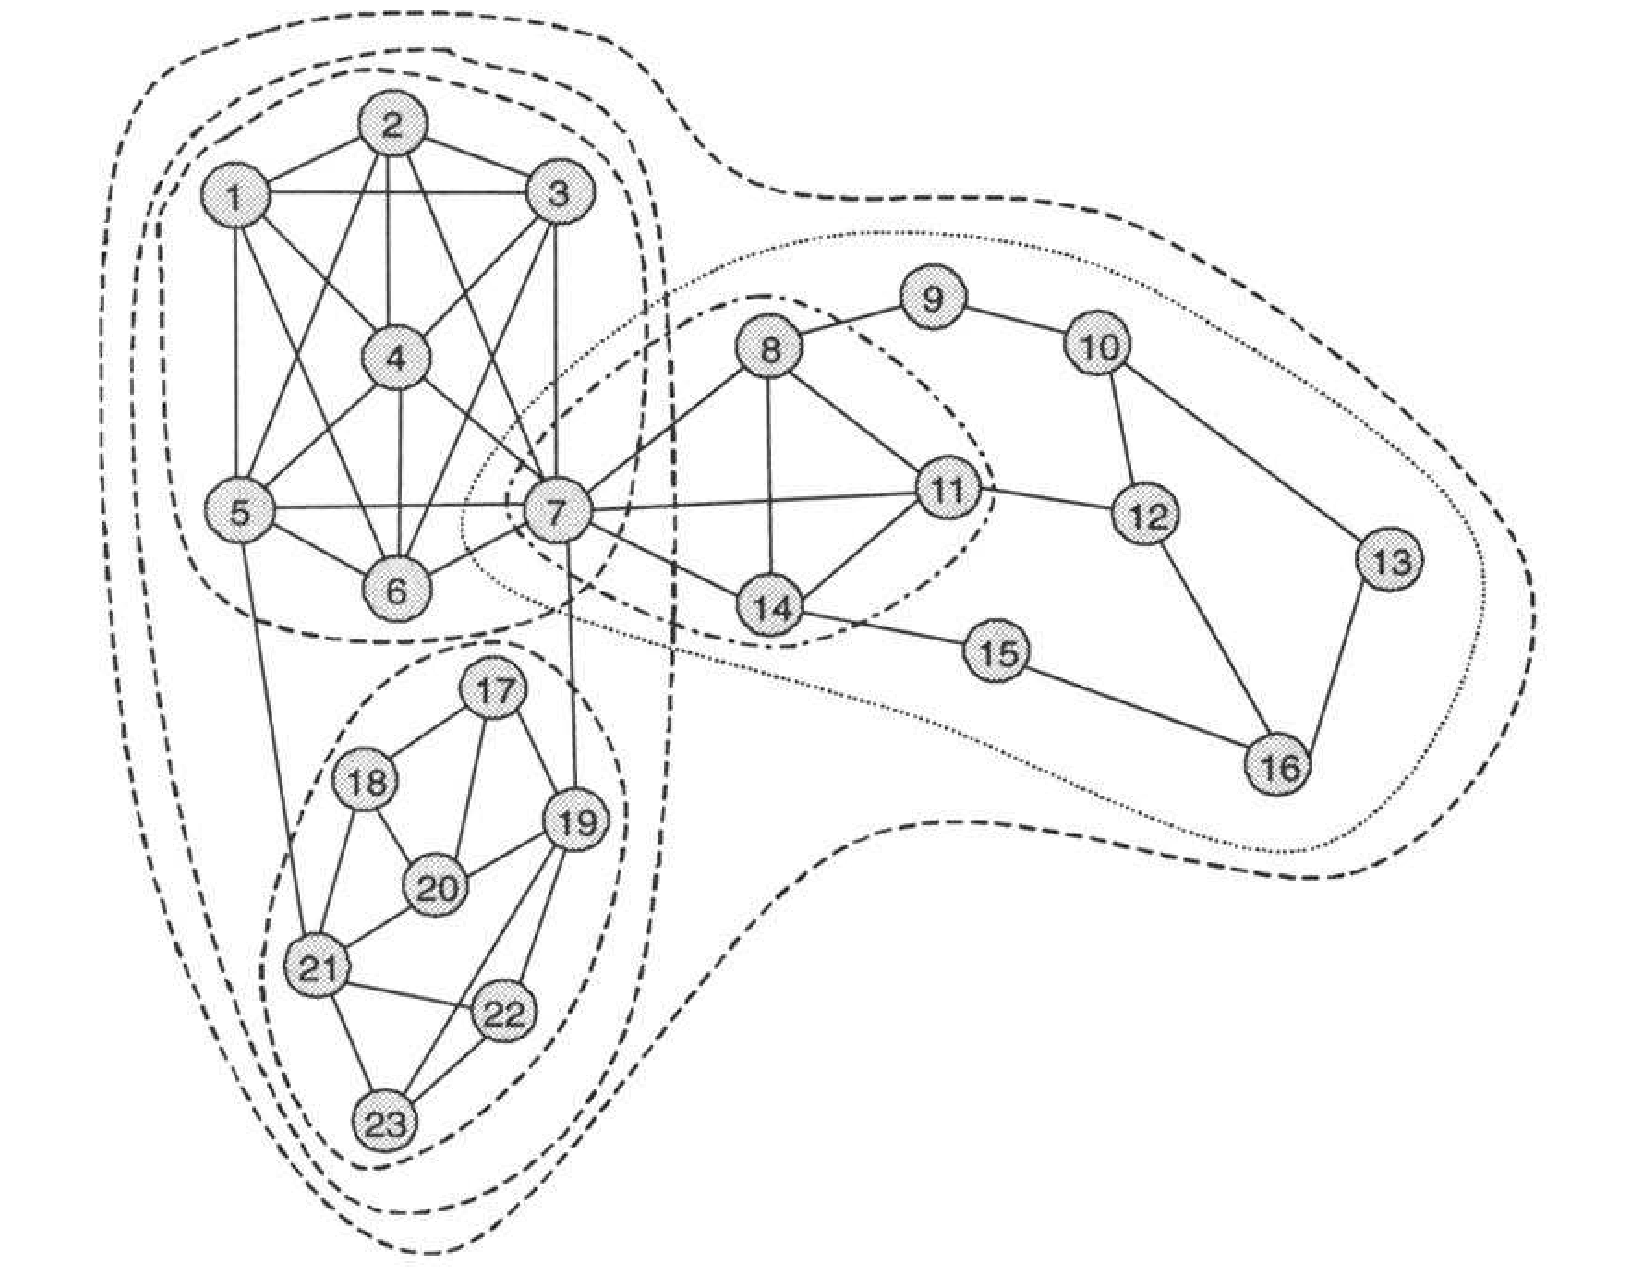
\includegraphics[width=0.6\textwidth]{../images/cblocks}\\

\newpage
\stitle{Cohesive blocks}
\begin{Myverb}
  blocks <- cohesive.blocks(cb)
  blocks

  summary(blocks)
  blocks$blocks
  lapply(blocks$blocks, "+", 1)
  blocks$block.cohesion #$
  plot(blocks, layout=layout.kamada.kawai,
       vertex.label.cex=2, vertex.size=15,
       vertex.label.color="black")
\end{Myverb}
   
\newpage
\stitle{Rapid prototyping}
\begin{narrow}{0cm}{15cm}
Weighted transitivity
\[ c(i)=\frac{\mathbf{A}^3_{ii}}{(\mathbf{A1A})_{ii}} \] \pause
\[ c_w(i)=\frac{\mathbf{W}^3_{ii}}{(\mathbf{WW_{\text{max}}W})_{ii}} \] \pause
\begin{Myverb}
  wtrans <- function(g) \{
    W <- get.adjacency(g, attr="weight")
    WM <- matrix(max(W), nrow(W), ncol(W))
    diag(WM) <- 0
    diag( W %*% W %*% W ) / 
       diag( W %*% WM %*% W)
  \}
\end{Myverb}
\end{narrow}

\newpage
\stitle{Rapid prototyping}
\begin{narrow}{0cm}{15cm}
Clique percolation, 
Palla et al., Nature 435 814--818, 2005\\
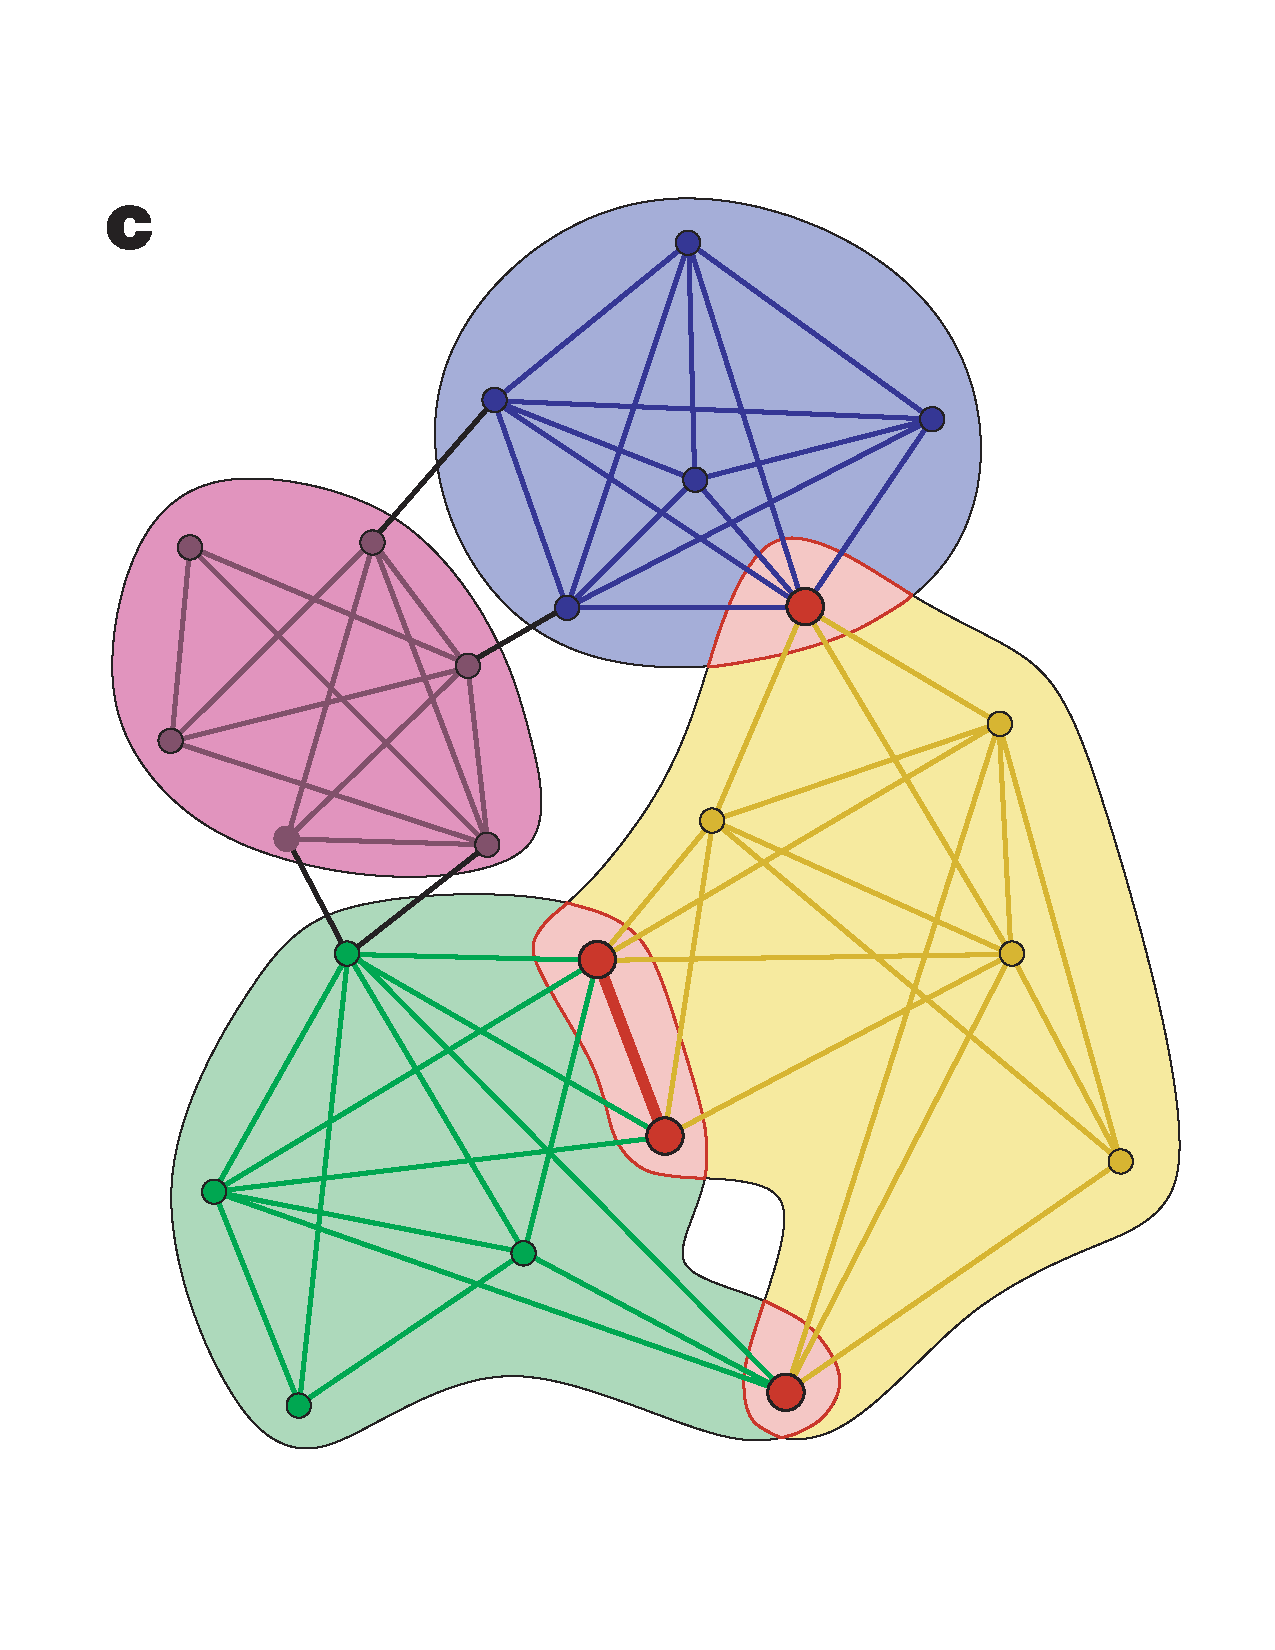
\includegraphics[width=\linewidth]{../images/vicsek}
\end{narrow}

\newpage
\stitle{Rapid prototyping, clique percolation}
\begin{narrow}{0cm}{15cm}
\vspace*{-10pt}
\begin{Myverb}
  clique.community <- function(graph, k) \{
   clq <- cliques(graph, min=k, max=k)
   edges <- c()
   for (i in seq(along=clq)) \{
     for (j in seq(along=clq)) \{
       if ( length(unique(c(clq[[i]], 
             clq[[j]]))) == k+1 ) \{
         edges <- c(edges, c(i,j)-1)
       \}
     \}
   \}
   clq.graph <- simplify(graph(edges))
   V(clq.graph)$name <- 
      seq(length=vcount(clq.graph))
   comps <- decompose.graph(clq.graph)
   
   lapply(comps, function(x) \{
     unique(unlist(clq[ V(x)$name ]))
   \})
  \}
\end{Myverb}
\end{narrow}

\newpage
\cstitle{Acknowledgement}

\begin{center}
\vfill
Tam\'as Nepusz\par\vfil
Peter McMahan, the BLISS, Walktrap and Spinglass projects\par\vfil
All the people who contributed code, sent bug reports, suggestions\par\vfil
The R project\par\vfil
Hungarian Academy of Sciences\par\vfil
The OSS community in general\par\vfill
\end{center}

\newpage
\cstitle{More information}
\begin{center}
\vfill
\centerline{\LARGE\url{http://igraph.sf.net}}\par\vspace*{3cm}
Please send your comments, questions, feature requests, code (!) to the
\url{igraph-help} mailing list. (See \textit{Community} on the
homepage.)\par\vfill
\end{center}

\end{document}
 
